\documentclass[11pt,a4paper]{article}
\usepackage[spanish,activeacute]{babel}
\decimalpoint
\usepackage[utf8]{inputenc}
\usepackage{listingsutf8}
\usepackage{amsmath}
\usepackage{amsfonts}
\usepackage{amssymb}
\usepackage{graphicx}
\usepackage{color}
\usepackage{listings}
\usepackage{amsthm}
\usepackage{caption}
\usepackage{subcaption}
\usepackage{dsfont}
\usepackage{comment}
\usepackage{enumerate}
\usepackage{mathtools,xparse}
\usepackage{ mathrsfs }
\usepackage{float}
\usepackage{listings}
\usepackage{xcolor}
\usepackage[ruled]{algorithm2e}

%% CODIGO PYTHON
\definecolor{codegreen}{rgb}{0,0.6,0}
\definecolor{codegray}{rgb}{0.5,0.5,0.5}
\definecolor{codepurple}{rgb}{0.58,0,0.82}
\definecolor{backcolour}{rgb}{0.93,0.93,0.93}

\lstdefinestyle{mystyle}{
    backgroundcolor=\color{backcolour},   
    commentstyle=\color{codegreen},
    keywordstyle=\color{magenta},
    numberstyle=\tiny\color{codegray},
    stringstyle=\color{codepurple},
    basicstyle=\ttfamily\footnotesize,
    breakatwhitespace=false,         
    breaklines=true,                 
    captionpos=b,                    
    keepspaces=true,                 
    numbers=left,                    
    numbersep=5pt,                  
    showspaces=false,                
    showstringspaces=false,
    showtabs=false,                  
    tabsize=2
}

\lstset{style=mystyle, inputencoding=utf8, extendedchars=true, literate={á}{{\'a}}1 {ó}{{\'o}}1 {é}{{\'e}}1 {ú}{{\'u}}1 {í}{{\'i}}1 {ñ}{{\~n}}1,}
%CODIGO PYTHON
\usepackage[left=2.3cm, right=2.1cm, top=2.35cm, bottom=2.35cm]{geometry}
%\renewcommand{\rmdefault}{mathpazo}
%\usepackage{mathpazo}

\usepackage[]{hyperref}
\hypersetup{
    pdftitle={Práctica 2 - MH},
    pdfauthor={Mario Muñoz Mesa},
    pdfsubject={ },
    pdfkeywords={keyword1, keyword2},
    bookmarksnumbered=true,     
    bookmarksopen=true,         
    bookmarksopenlevel=1,       
    colorlinks=true,   
    linkcolor=black,         
    pdfstartview=Fit,           
    pdfpagemode=UseOutlines,
    pdfpagelayout=TwoPageRight
}


\DeclarePairedDelimiter{\norm}{\lVert}{\rVert}
\NewDocumentCommand{\normL}{ s O{} m }{%
  \IfBooleanTF{#1}{\norm*{#3}}{\norm[#2]{#3}}_{L_2(\Omega)}%
}

\DeclareMathOperator*{\argmax}{arg\,max}
\DeclareMathOperator*{\argmin}{arg\,min}

\newtheorem{theorem}{Teorema}

\theoremstyle{definition}
\newtheorem{definition}{Definición}[section]


\newtheorem{proposition}{Proposición}[section]


\newtheorem{corolary}{Corolario}[section]


\newtheorem{lema}{Lema}[section]

	\newcommand{\R}{\mathbb{R}}
	\newcommand{\N}{\mathbb{N}}
	\newcommand{\C}{\mathbb{C}}


\title{
\normalfont \normalsize 
\textsc{\small METAHEURÍSTICAS} \\ [10pt]
	
	
\huge{\textbf{Práctica 2 - APC}}\\

\textsc{\small Grupo 1} \\ [10pt]

	}

\author{Mario Muñoz Mesa\\ mario43514@correo.ugr.es}
\date{\today}


\begin{document}
	\maketitle
	\newpage
	\renewcommand*\contentsname{Índice}	
	\tableofcontents
	
	\newpage
	
	\section{Descripción del problema.}
	Nos ocupamos del problema del Aprendizaje de Pesos en Características (APC). Plantea, en el contexto de un problema de clasificación, elegir o ajustar un vector de pesos $\textbf{w}=(w_1,\ldots, w_d)\in [0,1]^d$ asociado a las características en base a un criterio de mejora del clasificador. Hemos denotado con $d$ al número de características.\\
	
	En nuestro caso trabajaremos con clasificador tipo 1-NN, y el criterio será maximizar:
	$$F(\textbf{w}):=\alpha\cdot \text{tasa\_clas}(\textbf{w})+(1-\alpha ) \cdot \text{tasa\_red}(\textbf{w})$$
	donde
	$$\text{tasa-clas}:=100\frac{\text{nº instancias bien clasificadas en training}}{\text{nº instancias en training}}, \quad \quad \text{tasa-red}:=100\frac{\text{nº valores } w_i <0.2}{\text{nº características}}$$
	y $alpha=0.5$ que pondera la importancia entre el acierto y la reducción de características para el nuevo mejor clasificador que se pretende encontrar.\\
	
	De lo que nos ocupamos por tanto es de obtener $\argmax_{\textbf{w}\in [0,1]^d} F(\textbf{w})$ para un clasificador 1-NN que utilizará la distancia ponderada
	$$d_{\textbf{w}}(u,v)=\sqrt{\sum_{i=1}^d w_i(u_i-v_i)^2}, \quad u,v\in \R^d$$
	para clasificar. Queremos que aumente el acierto y reduzca el número de características, cualquier característica con peso menor estricto a 0.2 se descarta.
	
	
	\newpage
	\section{Descripción de la aplicación de los algoritmos empleados.}
	\subsection{Asociados al preprocesado y representación. P1.}
	Partimos de un conjunto de entrenamiento $T$ formado por instancias de una muestra. Cada instancia se ha representado mediante una estructura de datos \texttt{SampleElement} que recoge las valores de las características en un vector \texttt{vector<double>} y la clase como una cadena de caracteres.
	
	De esta forma, cada dataset se lee mediante la función \texttt{read\_arff} y lo almacenamos como un vector de elementos muestrales \texttt{vector<SampleElement>}. 
	
	Para la normalización utilizamos min-max normalization, se ha implementado en \texttt{normalization}.
	
	Las particiones para la validación cruzada $k-fold$ se realizan respetando la proporción de clases en cada partición, para ello cada elemento de una clase se va asignando a una partición de forma cíclica.
	
	La solución será un vector de pesos con valores entre 0 y 1, cada componente indica el peso de una característica, se representa como un \texttt{vector<double>}
	\subsection{Asociados al preprocesado y representación. P2.}
	Para los algoritmos genéticos se ha decidido representar cada cromosoma como un estructura de datos \texttt{Chromosome} que contiene un \texttt{vector<double>}, que representa los genes del cromosoma, junto con el el valor de la función objetivo asociado a ese cromosoma.
	
	Además se han definido los comparadores mayor, $>$, y menor, $<$. Un cromosoma es mayor a otro si su función objetivo es mayor, y menor si la función objetivo es menor.
	
	Para representar una población de cromosomas hacemos uso de una simple estructura de vector, \texttt{vector<Chromosome>}.
	\subsection{Funciones generales. P1.}
	Nuestro clasificador utiliza la distancia euclídea, para manejarla se han implementado dos funciones: \texttt{euclidean\_distance2} y \texttt{euclidean\_distance2\_w}.\\
	
	
	\begin{algorithm}[H]
		\caption{euclidean\_distance2}
		\KwIn{vector de reales $a$, vector de reales $b$}
		\KwOut{la distancia euclídea al cuadrado entre $a$ y $b$}
		\Begin{
			dist $\leftarrow$ 0
			
			\For { $i=0$ to $a.size()-1$ }{
				dist $\leftarrow$ dist + $(a[i]-b[i])^2$
			}
			\Return dist
		}
	\end{algorithm}~\\
	
	\begin{algorithm}[H]
		\caption{euclidean\_distance2\_w}
		\KwIn{vector de reales $a$, vector de reales $b$, vector de pesos $weights$}
		\KwOut{la distancia euclídea ponderada y al cuadrado entre $a$ y $b$}
		\Begin{
			dist $\leftarrow$ 0
			
			\For { $i=0$ \textbf{to} $a.size() -1$ }{
			\tcp{se descartan las características con peso < 2}	
				\If{$weights[i] \geq 0.2$}{ 
				dist $\leftarrow$ dist + $(a[i]-b[i])^2$
				}
			}
			\Return dist
		}
	\end{algorithm}~\\
	
	La función \texttt{euclidean\_distance2}  se utiliza exclusivamente para el cálculo de amigo y enemigo más cercano en el algoritmo Relief. Con \texttt{euclidean\_distance2\_w} calculamos la distancia ponderada descartando pesos menores a 0.2, se utiliza en 1-NN y Búsqueda Local.
	
	En ambos casos calculamos la distancia euclídea al cuadrado por motivos de eficiencia y porque lo que nos interesa es comparar distancias, y como la raíz cuadrada es una función creciente, si $a>b$ $\Rightarrow $ $\sqrt{a}>\sqrt{b}$, no hay inconveniente en trabajar con la distancia al cuadrado.
	
	El algoritmo 1-NN, haciendo uso de distancia ponderada, se ha implementado en \texttt{one\_NN}.\\
	
	\begin{algorithm}[H]
		\caption{one\_NN}
		\KwIn{elemento muestral $sam\_el$ a clasificar, conjunto de elementos muestrales sobre el que buscar el más cercano $sam\_elements$, vector de pesos $weights$}
		\KwOut{la clase o etiqueta del elemento más cercano, $min\_l$}
		\Begin{
			$min\_dist \leftarrow \infty$
			
			\For { $e$ \textbf{in} $sam\_elements$ }{
				$d\leftarrow$ euclidean\_distance2\_w(e.features, sam\_el.features, weights)
				
				\If{$d < min\_dist$}{
					$min\_l$ $\leftarrow$ e.label\\
					$min\_dist \leftarrow d$
				}
			}
			\Return min\_l
		}
	\end{algorithm}~\\
	
	La versión con leave-one-out, que se utiliza en Búsqueda Local, simplemente consiste en dejar un elemento fuera. \\
	
	\begin{algorithm}[H]
		\caption{one\_NN\_lo}
		\KwIn{elemento muestral $sam\_el$ a clasificar, conjunto de elementos muestrales sobre el que buscar el más cercano $sam\_elements$, vector de pesos $weights$, posición de elemento a dejar fuera $leave\_out$}
		\KwOut{la clase o etiqueta del elemento más cercano, $min\_l$}
		\Begin{
			$min\_dist \leftarrow \infty$
			
			\For { $i=0$ \textbf{to} $sam\_elements.size()-1$ }{
			\If{$i\neq leave\_out$}{
				$d\leftarrow$ euclidean\_distance2\_w(sam\_elements[i].features, sam\_el.features, weights)
				
				\If{$d < min\_dist$}{
					$min\_l$ $\leftarrow$ sam\_elements[i].label\\
					$min\_dist \leftarrow d$
				}
			}
			}
			\Return min\_l
		}
	\end{algorithm}
	
	\subsection{Funciones generales. P2.}
		El operador de selección utiliza un torneo binario; escoge dos cromosomas de la población aleatoriamente y devuelve el que de mayor valor en la función objetivo.\\
		
		\begin{algorithm}[H]
		\caption{selection}
		\KwIn{Población de cromosomas $population$}
		\KwOut{El cromosoma elegido por torneo binario}
		\Begin{
			$pop\_size\_1 \leftarrow population.size()-1$
			
			$c1 \leftarrow population[random(0,pop\_size\_1)]$
			
			$c1 \leftarrow population[random(0,pop\_size\_1)]$
			
			\If{$c1.obj > c2.obj$}{
				\Return $c1$
			}
			\Else{
				\Return $c2$
			}

		}
	\end{algorithm}~\\
		
		El operador de cruce blx toma dos cromosomas y genera dos descendientes. Cada gen de cada cromosoma descendiente es generado aleatoriamente en intervalo $[c_{min}-I\cdot \alpha, c_{max}+I\cdot \alpha]$ donde $c_{min}$ y $c_{max}$ son el mínimo y máximo entre los dos genes correspondientes de los cromosomas iniciales, $I=c_{max}-c_{min}$ y $\alpha=0.3$. Los valores resultantes en cada gen se restringen a $[0,1]$.\\
		
	\begin{algorithm}[H]
	\caption{blx\_cross}
		\KwIn{Dos cromosomas $p1$ y $p2$}
		\KwOut{Los dos cromosomas descendientes $d1$ y $d2$}
		\Begin{
			$pgenes\_size \leftarrow p1.genes.size()$
			
			\For{$i=0$ \textbf{to} $pgenes\_size$}{
				$c_{min} \leftarrow \min\{p1.genes[i], p2.genes[i]\}$
				
				$c_{max} \leftarrow \max\{p1.genes[i], p2.genes[i]\}$
				
				$I\alpha \leftarrow (c_{max} - c_{min}) * 0.3$
				
				$d1.genes[i] \leftarrow random(c_{min}-I\alpha, c_{max}+ I\alpha)$
				
				$d2.genes[i] \leftarrow random(c_{min}-I\alpha, c_{max}+ I\alpha)$
				
				\tcp{restringimos a intervalo [0,1]}
				$restrict\_to\_0\_1(d1.genes[i])$
				
				$restrict\_to\_0\_1(d2.genes[i])$
			}
			\tcp{para evitar evaluaciones de f.obj redundantes antes de la mutación}
			$d1.obj \leftarrow -1$
			
			$d2.obj \leftarrow -1$
			
			\Return{$d1$, $d2$}
		}
	\end{algorithm}~\\
	
	El operador de cruce aritmético toma dos cromosomas y genera también dos descendientes. En este caso para cada descendiente en vez de tomar $\alpha=0.5$ se toma un $\alpha$ aleatorio entre 0 y 1 (concretamente entre 0.01 y 0.99 en la implementación), esto se hace para evitar la generación de descendientes idénticos.\\
	
	\begin{algorithm}[H]
	\caption{arith\_cross}
		\KwIn{Dos cromosomas $p1$ y $p2$}
		\KwOut{Los dos cromosomas descendientes $d1$ y $d2$}
		\Begin{
			$gen\_size \leftarrow p1.genes.size()$
			
			$\alpha \leftarrow random(0.01,0.99)$
			
			\For{$i=0$ \textbf{to} $gen\_size$}{
				$d1.genes[i] \leftarrow \alpha * p1.genes[i] + (1-\alpha) * p2.genes[i]$
			}
			
			$\alpha \leftarrow random(0.01,0.99)$
			
			\For{$i=0$ \textbf{to} $gen\_size$}{
				$d2.genes[i] \leftarrow \alpha * p1.genes[i] + (1-\alpha) * p2.genes[i]$
			}
			
			
			\tcp{para evitar evaluaciones de f.obj redundantes antes de la mutación}
			
			$d1.obj \leftarrow -1$
			
			$d2.obj \leftarrow -1$
			
			\Return{$d1$, $d2$}
		}
	\end{algorithm}~\\
	
	El operador de mutación coincide con el de generación de vecinos en la BL, introduce una perturbación con una normal de media 0 y desviación típica $0.3$.  \\
	
	\begin{algorithm}[H]
		\caption{mutation}
		\KwIn{vector de pesos $weights$, índice a mutar $i$, distribución normal $n\_dist$}
		\Begin{
		$weights[i] \leftarrow weights[i] + e\in \mathcal{N}_{n\_dist}(0,0.3)$\\
		\If{$weigths[i]>1$}{
			$weights[i]\leftarrow 1$		
		}
		\Else{
			\If{$weights[i]<0$}{
				$weights[i]\leftarrow 0$			
			}		
		}
		}
	\end{algorithm}~\\
	
	Para realizar un número de mutaciones sobre una población de cromosomas se define la función \texttt{mutate\_pop}, ésta controla que no se repitan las mutaciones sobre un gen de un cromosoma.\\
	
	\begin{algorithm}[H]
		\caption{mutate\_pop}
		\KwIn{vector de cromosomas $population$, número de mutaciones a realizar $num\_muts$}
		\Begin{
		$pop\_size\_1 \leftarrow population.size() - 1 $
		
		$genes\_size\_1 \leftarrow num\_of\_genes - 1$  \tcp{equivale a num\_feats-1 en implementación}
		
		$mutated \leftarrow \{\}$
		
		$muts \leftarrow 0$
		
		\While{$muts < num\_muts$}{
			$chr\_i \leftarrow random(0,pop\_size\_1)$
			
			$gen\_i \leftarrow random(0,genes\_size\_1)$
			
			\If{$\{chr\_i,\ gen\_i \}$ $\notin$ $mutated$}{
				$mutation(population[chr\_i].genes,\ gen\_i,\ \mathcal{N}(0, 0.3))$
				
				$muts \leftarrow muts +1 $
				
				$mutated \leftarrow mutated \cup \{chr\_i,\ gen\_i \}$ 
				
				$population[chr\_i].obj \leftarrow -1$
				
			}
		
		}
		}
	\end{algorithm}~\\
	
		Para evaluar la función objetivo asociada a los genes de un cromosoma y asignarlo al cromosoma se ha creado la función \texttt{obj\_to\_chromosome}:\\
		
		\begin{algorithm}[H]
		\caption{obj\_to\_chromosome}
		\KwIn{cromosoma $c$, vector de elementos muestrales $training$}
		\Begin{
		
		\For{$i=0$ \textbf{to} $training.size()$}{
			$class\_labels.push\_back(\ one\_NN\_lo(training[i], training, c.genes, i)\ )$
		}
		
		$c.obj \leftarrow obj\_function(class\_rate(class\_labels, training), \ red\_rate(c.genes))$
		}
	\end{algorithm}
	
	\subsection{Función objetivo.}
	Para el cálculo de las tasas se han implementado las funciones \texttt{class\_rate} y \texttt{red\_rate} que simplemente implementan la propia de definición de tasa-class y tasa-red.\\
	
	\begin{algorithm}[H]
		\caption{class\_rate}
		\KwIn{vector con clases o etiquetas de elementos clasificados $class\_labels$, elementos de test $test$}
		\KwOut{el porcentaje de acierto}
		\Begin{
			$n\leftarrow 0$\\
  			$class\_labels\_s \leftarrow class\_labels.size()$
  			
			\For { $i=0$ \textbf{to} $class\_labels\_s-1$ }{
			\If{$class\_labels\_s[i] == test[i].label$}{
				$n\leftarrow n+1$
			}

			}
			
			\Return $100\frac{n}{class\_labels\_n}$
		}
	\end{algorithm}~\\
	
	\begin{algorithm}[H]
		\caption{red\_rate}
		\KwIn{vector de pesos $weights$}
		\KwOut{el porcentaje de reducción}
		\Begin{
			$feats\_reduced \leftarrow 0$
			
			\For { $w$ \textbf{in} $weights$ }{
			\If{$w < 0.2$}{
				$feats\_reduced \leftarrow feats\_reduced+1$
			}

			}
			
			\Return $100\frac{feats\_reduced}{initial\_number\_of\_features}$
		}
	\end{algorithm} ~\\
	
	La función objetivo, teniendo en cuenta que trabajamos con $\alpha = 0.5$, nos quedaría:\\
	
	\begin{algorithm}[H]
		\caption{obj\_function}
		\KwIn{tasa de clasificación $class\_rate$, tasa de reducción $red\_rate$}
		\KwOut{el valor de la función objetivo o fitness}
		\Begin{
			
			\Return $\alpha \cdot class\_rate + (1-\alpha) \cdot red\_rate$
		}
	\end{algorithm}
	
	\section{Descripción de los algoritmos.}
	\subsection{Algoritmos genéticos.}
	Los algoritmos genéticos generacionales y estacionarios que se han implementado siguen un cierto esquema:
	\begin{enumerate}
		\item Generar una población inicial de 30 cromosomas con valores de distribución uniforme $\mathcal{U}(0,1)$ para los genes.
		\item Seleccionar los cromosomas a los que se aplicará un cruce, ya sean 2 en el caso de AGE o igual a la población inicial en el caso de AGG.
		\item Cruzar los individuos ya sea con cruce blx o cruce aritmético en base a una probabilidad de cruce.
		\item Mutar ciertos cromosomas en base a una probabilidad de mutación.
		\item Reemplazar la población antigua por la obtenida, ya sea conservando el de mejor función objetivo de la población antigua como en el caso de AGG, o sustituyendo en la población antigua los peores que tengan peor función objetivo que alguno de la nueva población generada, se sustituye por el que lo supera; este es el caso de AGE.% los que tengan peores valores de función objetivo por los que se han obtenido que superen en función objetivo. %conservando los que tengan mayores valores en función objetivo como en el caso de AGE.
		\item Volver al paso 2 hasta una condición de parada.
	\end{enumerate}
	
	La condición de parada consiste en no realizar más de 15000 evaluaciones de la función objetivo.
	
	La operación de selección, mutación y los tipos de cruces son los descritos en la sección 2.4.~\\
	
	\textit{Nota:} en la implementación/código correspondiente a los pseudocódigos mostrados a continuación se incluyó una opción de cruce adicional para SBX2, ésta fue añadida a posteriori para el experimento extra.
	
	\subsubsection{Algoritmo genético generacional (AGG).}
	Para los algoritmos genéticos generacionales la probabilidad de cruce es 0.7 y la probabilidad de mutación 0.1 por cromosoma.
	
	Para evitar la excesiva generación de aleatorios se estima previamente el número de cruces y mutaciones esperados.
	
	\begin{itemize}
	\item El número de cruces esperado es $\approx \frac{0.7\cdot 30}{2}\approx 11$. 
	
	\item El número de mutaciones esperado es $\frac{0.1}{\text{número genes}}$ por gen, se realizarán por tanto $\frac{0.1}{\text{número genes}} \cdot 30 \cdot \text{número genes}=3$ mutaciones.
	\end{itemize}
	
	Para conservar el elitismo la mejor solución de la población anterior, $s_1$, reemplaza a la peor de la nueva población si $s_1$ es mejor que la mejor solución de la nueva población.\\
	
	\begin{algorithm}[H]
		\caption{agg}
		\KwIn{vector de elementos muestrales $training$, entero que indica el tipo de cruce a utilizar $cross\_type$}
		\KwOut{los genes del mejor cromosoma encontrado}
		\Begin{
			$pop\_size \leftarrow 30$
			
			%$exp\_num\_crosses \leftarrow round(0.7 * pop\_size / 2)$
			$exp\_num\_crosses,\ exp\_num\_muts \leftarrow round(0.7 * pop\_size / 2),\ round( 0.1*pop\_size)$ 
			
			$chr\_to\_cross \leftarrow 2*exp\_num\_crosses$
			
			%$exp\_num\_muts \leftarrow round( 0.1*pop\_size)$
			
			$evals\leftarrow 0$
			
			\iffalse
			\If{$cross\_type == 0$}{
				$cross\leftarrow blx\_cross$
			}
			\Else{
				\If{$cross\_type == 1$}{
					$cross\leftarrow arith\_cross$				
				}
			}
			\fi
			$cross\_type \leftarrow [blx\_cross,\ arith\_cross][cross\_type]$
			
			\tcp{1. se genera población inicial}
			\For{$i=0$ \textbf{to} $pop\_size$}{
				\For{$j=0$ \textbf{to} $num\_feat$}{
					$population[i].genes[j] \leftarrow random(0,1)$
				}
				
				$obj\_to\_chromosome(population[i], training)$
				
				$evals\leftarrow evals+1$
			}
			%\tcp{se guarda el cromosoma con mayor función objetivo en la población}
			$best\_parent \leftarrow \argmax\{c.obj \ : \ c\in population\}$ \tcp{el de mayor f.obj}
			
			\While{$evals < 15000$}{
			\tcp{2, 3. se seleccionan población que se va a cruzar y se cruza}
				\For{$i=0$ \textbf{to} $chr\_to\_cross$ \textbf{step} $=2$}{
					$sel1\leftarrow selection(population)$
					
					$sel2 \leftarrow selection(population)$
					
					%$descendents \leftarrow cross(sel1, sel2)$
					
					$inter\_population[i],\  inter\_population[i+1] \leftarrow cross(sel1, sel2)$
					
					%$i \leftarrow i+2$
				}
				\tcp{2. se selecciona población restante que no se cruza}
				\For{$i=chr\_to\_cross$ \textbf{to} $pop\_size$}{
				$inter\_population[i] \leftarrow selection(population)$
				}
				\tcp{4. se realizan exp\_num\_muts mutaciones de genes de cromosomas de forma aleatoria}
				$mutate\_pop(inter\_population,\ exp\_num\_ muts)$
				
				\tcp{5. se reemplaza la población}
				$population\leftarrow inter\_population$
				
				\For{$c$ \textbf{in} $population$}{
					 \If{$c.obj == -1$}{
					 	$obj\_to\_chromosome(c,\ training)$
					 	
					 	$evals\leftarrow evals+1$
					 }
				}
				\tcp{5. se mantiene el mejor}
				$best\_descendent \leftarrow \argmax\{c.obj \ : \ c\in population\}$
				
				\If{$best\_parent > best\_descendent$}{
					$\argmin\{c.obj \ : \ c\in population\} \leftarrow best\_parent$
				}
				\Else{
					$best\_parent \leftarrow best\_descendent$
				}
			}
			\Return{$(\argmax\{c.obj \ : \ c\in population\}).genes$}
			}
			
	\end{algorithm}
	
	\subsubsection{Algoritmo genético estacional (AGE).}
	Para los algoritmos genéticos estacionales la probabilidad de cruce es 1, se cruzan los dos cromosomas que se seleccionan.
	
	 La probabilidad de mutación es 0.1 por cromosoma al igual que en el caso generacional, en este caso, al partir de solo 2 cromosomas tras la selección, el número esperado de mutaciones es menor a 1 por lo que sí generaremos el aleatorio en cada caso.
	 
	 En este caso las dos soluciones generadas compiten con las anteriores sustituyendo a las peores en caso de mejorarlas.\\
	 
	 \begin{algorithm}[H]
		\caption{age}
		\KwIn{vector de elementos muestrales $training$, entero que indica el tipo de cruce a utilizar $cross\_type$}
		\KwOut{los genes del mejor cromosoma encontrado}
		\Begin{
			$pop\_size \leftarrow 30$

			$evals\leftarrow 0$
			
			$cross\_type \leftarrow [blx\_cross,\ arith\_cross][cross\_type]$
			
			\tcp{1. se genera población inicial}
			\For{$i=0$ \textbf{to} $pop\_size$}{
				\For{$j=0$ \textbf{to} $num\_feat$}{
					$population[i].genes[j] \leftarrow random(0,1)$
				}
				
				$obj\_to\_chromosome(population[i], training)$
				
				$evals\leftarrow evals+1$
			}
			
			\While{$evals < 15000$}{
			\tcp{2, 3. se seleccionan población que se va a cruzar y se cruza}

				$sel1\leftarrow selection(population)$
					
				$sel2 \leftarrow selection(population)$
					
				$inter\_population[0],\  inter\_population[1] \leftarrow cross(sel1, sel2)$

				\tcp{4. se realizan mutaciones con probabilidad de mutación de 0.1 por cromosoma}
				\For{$i=0$ \textbf{to} 2}{
					\If{$random(0,1)$ $\leq$ $0.1$}{
						$mutation(inter\_population[i].genes,\ random(0,\ num\_feats-1),\ \mathcal{N}(0,0.3))$
						
						$inter\_population[i].obj \leftarrow -1$
					}
				}
				
				\tcp{se evalúa f.obj en población intermedia}

				\For{$c$ \textbf{in} $inter\_population$}{
					 \If{$c.obj == -1$}{
					 	$obj\_to\_chromosome(c,\ training)$
					 	
					 	$evals\leftarrow evals+1$
					 }
				}
				\tcp{5. sustituir peores elementos de la población por los de pob. intermedia si son mejores}

				\For{$c$ \textbf{in} $inter\_population$}{
					\If{$\argmin\{c.obj \ : \ c\in population\} < c$}{
					$\argmin\{c.obj \ : \ c\in population\} \leftarrow c$
					}
				}
			}
			\Return{$(\argmax\{c.obj \ : \ c\in population\}).genes$}
			}
			
	\end{algorithm}
	\subsection{Algoritmos meméticos.}
	Los algoritmos meméticos consisten en aplicar un algoritmo genético realizando BL de baja intensidad sobre el total o un sobjunto de la población cada 10 generaciones en nuestro caso.
	
	
	La búsqueda local de baja intensidad implementada equivale a una adaptación de la desarrollada en la práctica 1.b, donde ahora se indica el cromosoma con el que comenzar la búsqueda, el máximo número de vecinos a evaluar será $2\cdot n$ con $n$ el tamaño de cromosoma (su número de genes), y el número de evaluaciones comienza a partir del dado como argumento por referencia.\\
	
	
	
	\begin{algorithm}[H]
		\caption{li\_ls}
		\KwIn{conjunto de elementos muestrales $training$, cromosoma $c$, evaluaciones de f.obj ya realizadas $obj\_eval\_count$}
		\Begin{
			$n\leftarrow c.genes.size()$ \tcp{equivale a number\_of\_features}
			
			\tcp{inicialización de índices de genes}
			\For{$i=0$ \textbf{to} $n$}{
				$comp\_indexes.push\_back()$
			}
			$best\_obj \leftarrow c.obj$
			
			$gen\_neighbours\leftarrow 0$
			
			
			$mod\_pos \leftarrow 0$
			
			\While{$gen\_neighbours < 2*n$ \textbf{and} $obj\_eval\_count < 15000$}{
			\tcp{aleatorizamos componentes a mutar si se han recorrido todas o se mejoró f.obj}
			\If{$new\_best\_obj$ \textbf{or} $mod\_pos \% number\_of\_features == 0$}{
				$new\_best\_obj \leftarrow false$\\
				$shuffle(comp\_indexes)$\\
				$mod\_pos \leftarrow 0$
			}
			\tcp{Se toma componente a mutar y se muta}
			$comp\_to\_mut \leftarrow comp\_indexes[mod\_pos \% n]$
			
			$muted\_c \leftarrow c$
			
			$mutation(muted\_c.genes,\  comp\_to\_mut,\  \mathcal{N}(0,0.3))$
			
			$gen\_neighbours \leftarrow gen\_neighbours + 1$

			\tcp{se asigna f. obj a cromosoma con los pesos mutados (con leave one out)}
			$obj\_to\_chromosome(muted\_c,\ training)$
			
			\tcp{si se ha mejorado, actualizamos mejor objetivo, cromosoma y vecinos generados}
			\If{$muted\_c.obj>best\_obj$}{
				$c \leftarrow muted\_c$\\
				$best\_obj \leftarrow obj$\\
				%$gen\_neighbours \leftarrow 0$\\
				$new\_best\_obj \leftarrow true$
			}
			
			$obj\_eval\_count\leftarrow obj\_eval\_count+1$\\
			$mod\_pos\leftarrow mod\_pos +1$
			}
					
		}
		
	\end{algorithm}~\\
	
	Los algoritmos meméticos implementados se basan en AGG-BLX que fue el algoritmo generacional que mejor resultados proporcionó. 
	
	La forma de aplicar la búsqueda local de baja intensidad varía en las 3 versiones implementadas. Para no repetir pseudocódigo se indica solo la parte de pseudocódigo que difiere de AGG-BLX.~\\
	
	\textit{Nota:} en la implementación/código correspondiente a los pseudocódigos mostrados a continuación se incluyó un argumento adicional para indicar cruce BLX o SBX2, éste fue añadido a posteriori para el experimento extra.~\\
	
	En AM-(10,1.0) se aplica la búsqueda local a todos los cromosomas de la población.\\
	
	\begin{algorithm}[H]
		\caption{am\_1010}
		\KwIn{vector de elementos muestrales $training$}
		\KwOut{los genes del mejor cromosoma encontrado}
		\Begin{
			$pop\_size \leftarrow 10$
			
			$\ldots$
			
			$cross\_type\leftarrow  blx\_cross$
			
			$\ldots$
			
			\While{$evals < 15000$}{
			
			$\ldots$
			
			\If{$generation \% 10 == 0$}{
				\For{$c$ \textbf{in} $ population$}{
					$li\_ls(training,\ c,\ evals)$
				}
			}
			
			}
			$\ldots$
			%\Return{$(\argmax\{c.obj \ : \ c\in population\}).genes$}
			}
			
	\end{algorithm}~\\
	
	En AM-(10,0.1) se aplica la búsqueda local a cada cromosoma con probabilidad 0.1. Esto es, se aplica sobre 1 cromosoma.\\
	
	\begin{algorithm}[H]
		\caption{am\_1001}
		\KwIn{vector de elementos muestrales $training$}
		\KwOut{los genes del mejor cromosoma encontrado}
		\Begin{
			$pop\_size \leftarrow 10$
			
			$\ldots$
			
			$cross\_type\leftarrow  blx\_cross$
			
			$\ldots$
			
			\While{$evals < 15000$}{
			
			$\ldots$
			
			\If{$generation \% 10 == 0$}{
				$li\_ls(training,\ population[random(0,\ pop\_size-1),\ evals)$
			}
			
			}
			$\ldots$
			%\Return{$(\argmax\{c.obj \ : \ c\in population\}).genes$}
			}
			
	\end{algorithm}~\\
	
	En AM-(10,0.1 mej) el cromosoma sobre el que aplica la búsqueda local  ya no es aleatorio, se aplica sobre el mejor de la población.\\
	
	\begin{algorithm}[H]
		\caption{am\_1001\_mej}
		\KwIn{vector de elementos muestrales $training$}
		\KwOut{los genes del mejor cromosoma encontrado}
		\Begin{
			$pop\_size \leftarrow 10$
			
			$\ldots$
			
			$cross\_type\leftarrow  blx\_cross$
			
			$\ldots$
			
			\While{$evals < 15000$}{
			
			$\ldots$
			
			\If{$generation \% 10 == 0$}{
				$li\_ls(training,\ \argmax\{c.obj \ : \ c\in population\},\ evals)$ 
			}
			
			}
			$\ldots$
			%\Return{$(\argmax\{c.obj \ : \ c\in population\}).genes$}
			}
			
	\end{algorithm}
\iffalse
	\subsection{RELIEF (Greedy).}
	Este algoritmo será el de comparación. El objetivo es generar un vector de pesos a partir de las distancias de cada ejemplo o elemento al amigo (misma clase) y enemigo (clase distinta) más cercano.
	
	La idea subyacente es, para cada característica, premiar en peso la lejanía de un ejemplo a su enemigo más cercano (separa bien), y penalizar la lejanía de un ejemplo a su amigo más cercano.
	
	Se comienza con vector de pesos 0. Se recorren los elementos de entrenamiento, identificando enemigo y amigo más cercano, y se actualizan las componentes de los pesos sumando la distancia del enemigo más cercano y restando la del amigo más cercano en cada característica. Luego se restringen los pesos a $[0,1]$ truncando los valores negativos a 0 y normalizando el resto dividiendo por el máximo peso en el vector de pesos.
	
	Para la implementación se ha creado previamente la función \texttt{closest\_friend\_enemy} que busca el amigo y enemigo más cercanos a un elemento.~\\
	
	\begin{algorithm}[H]
		\caption{closest\_friend\_enemy}
		\KwIn{posición del elemento $pos$, conjunto de entrenamiento $training$, elemento que será el amigo más cercano $friend\_e$, elemento que será el enemigo más cercano $enemy\_e$}
		\Begin{
			$min\_friend\_d \leftarrow \infty$\\
			$min\_enemy\_d \leftarrow \infty$
			
			\For{$i \in \{0,\ldots ,pos-1, pos+1,\ldots , training.size()-1\}$}{
				$distance\leftarrow  euclidean\_distance2(training[i].features, training[pos].features) $
				
			\If{elemento i y elemento pos son amigos}{
				\If{$distance < min\_friend\_d$}{
					$min\_friend\_d \leftarrow distance$\\
					$min\_friend\_p \leftarrow i$
				}
			}
			\Else{
				\If{$distance < min\_enemy\_d$}{
					$min\_enemy\_d \leftarrow distance$\\
					$min\_enemy\_p \leftarrow i$
				}
			}
		}
		$friend\_e \leftarrow training[min\_friend\_p]$\\
		$enemy\_e \leftarrow training[min\_enemy\_p]$\\
		}
	\end{algorithm}~\\
	
	
	El agoritmo RELIEF:~\\
	
	\begin{algorithm}[H]
		\caption{relief}
		\KwIn{conjunto de elementos muestrales $training$}
		\KwOut{vector de pesos $weights$}
		\Begin{
			$weights \leftarrow (0,\ldots ,0)$\\
			\tcp{se va buscando enemigo y amigo más cercano para cada elemento}
			\For{$i=0$ \textbf{to} $training.size()-1$}{
				$closest\_friend\_enemy(i, training, friend, enemy) $\\
			\tcp{se actualizan los pesos}
			\For{$j=0$ \textbf{to} $num\_feats-1$}{
				\If{$distance < min\_friend\_d$}{
					$weights[j]\leftarrow weights[j]+|training[i].features[j]-enemy.features[j]| - |training[i].features[j]-friend.features[j]|$
				}
			}

			}
			$max\_weight \leftarrow \max_{i\in \{0,\ldots , num\_feats -1\} } weights[i]$\\
			\tcp{se restringe a [0,1]}
			\For{$j=0$ \textbf{to} $num\_feats$}{
				\If{$weights[j] < 0$}{
					$weights[j] \leftarrow 0$				
				}
				\Else{
					$weights[j]\leftarrow \frac{weights[j]}{max\_weight}$				
				}			
			}
			\Return weights

		}
	\end{algorithm}
	\subsection{Búsqueda Local.}
	Para la Búsqueda Local se emplea la estrategia del primer mejor. \iffalse La idea es escoger la primera solución vecina (vector de pesos) que mejore la función objetivo actual.\fi La idea es generar soluciones (vectores de pesos) vecinas hasta encontrar la primera mejor que la actual, en ese caso se sustituye la actual por la encontrada. Este proceso es iterativo.
	
	Para ello se parte de una solución (vector de pesos) inicial; se toman valores de una distribución uniforme $\mathcal{U}(0,1)$.
	
	Para generar las soluciones vecinas, se va eligiendo una componente aleatoria sin repetición. Las soluciones vecinas se generan mutando el vector de pesos actual al sumar un elemento de una distribución normal de media 0 y desviación típica 0.3 (pesos fueras del rango [0,1] se truncan). Si se mejora la función objetivo con el nuevo vector de pesos, éste pasará a ser el actual. Además, en ese caso, o en el caso de haber recorrido todas las componentes, se establece un nuevo orden aleatorio de las componentes a recorrer.
	
	Este proceso se repite iterativamente hasta alcanzar 15000 evaluaciones de la función objetivo o hasta la generación de un número de vecinos igual a 20 veces el número de características.
	

	Para representar los índices de componentes del vector de pesos, que eventualmente se mezclan según lo anterior, se ha construido un vector de enteros. Este vector junto con el vector de pesos se inicializan en la función \texttt{rand\_init\_sol\_gen\_indexes}~\\
	
	\begin{algorithm}[H]
		\caption{rand\_init\_sol\_gen\_indexes}
		\KwIn{vector en el que inicializar los pesos $weights$, vector de índices $indexes$}
		\Begin{
			\For{$i=0$ \textbf{to} $number\_of\_features-1$}{
				$weights.push\_back(e\in \mathcal{U}(0,1))$\\
				$indexes.push\_back(i)$
			}

		}
	\end{algorithm}~\\
	
	También hemos construido una función que realiza la mutación en el vector de pesos:~\\
	
	\begin{algorithm}[H]
		\caption{mutation}
		\KwIn{vector de pesos $weights$, índice a mutar $i$, distribución normal $n\_dist$}
		\Begin{
		$weights[i] \leftarrow weights[i] + e\in \mathcal{N}_{n\_dist}(0,0.3)$\\
		\If{$weigths[i]>1$}{
			$weights[i]\leftarrow 1$		
		}
		\Else{
			\If{$weights[i]<0$}{
				$weights[i]\leftarrow 0$			
			}		
		}
		}
	\end{algorithm}~\\
	
	Y una función que clasifica un conjunto de elementos mediante leave one out, con distancia ponderada, y obtiene el correspondiente valor de la función objetivo para esa clasificación:~\\ 
	
	\begin{algorithm}[H]
		\caption{classifyloo\_and\_objf}
		\KwIn{elementos de entrenamiento conjunto de entrenamiento $training$, vector de pesos $weights$, vector a contener las etiquetas de clasificación $class\_labels$}
		\KwOut{el valor de la función objetivo de la clasificación, $obj$}
		\Begin{
		\For{$k=0$ \textbf{to} $training.size()-1$}{
			$class\_labels.push\_back(one\_NN\_lo(training[k], training, weights, k))$
		}
		$obj\leftarrow obj\_function(class\_rate(class\_labels, training), red\_rate(weights))$\\
		$class\_labels.clear()$
		
		\Return $obj$
		
		}
	\end{algorithm}~\\
	
	Finalmente tenemos la función que realiza la búsqueda local:~\\
	
	\begin{algorithm}[H]
		\caption{local\_search}
		\KwIn{conjunto de elementos muestrales $training$}
		\KwOut{mejor vector de pesos alcanzado $weights$}
		\Begin{
			$rand\_init\_sol\_gen\_indexes(best\_weights, comp\_indexes)$\\
			\tcp{clasificamos con los mejores pesos hasta el momento mediante leave one out, y obtenemos valor de la función objetivo}
			$best\_obj \leftarrow classifyloo\_and\_objf(training, best\_weights, class\_labels)$\\ ~\\
			
			\While{$gen\_neighbours < max\_gen\_neighbours$ \textbf{and} $obj\_eval\_count < max\_objf\_evals$}{
			\tcp{aleatorizamos componentes a mutar si se han recorrido todas o se mejoró f.obj}
			\If{$new\_best\_obj$ \textbf{or} $mod\_pos \% number\_of\_features == 0$}{
				$new\_best\_obj \leftarrow false$\\
				$shuffle(comp\_indexes)$\\
				$mod\_pos \leftarrow 0$
			}
			\tcp{Se toma componente a mutar y se muta}
			$comp\_to\_mut \leftarrow comp\_indexes[mod\_pos \% number\_of\_features]$
			
			$muted\_weights \leftarrow best\_weights$
			
			$mutation(muted\_weights, comp\_to\_mut, n\_dist)$\\
			
			$gen\_neighbours \leftarrow gen\_neighbours +1$\\
			\tcp{clasificamos con los nuevos pesos mutados mediante leave one out, y obtenemos valor de la función objetivo}
			$obj \leftarrow classifyloo\_and\_objf(training, muted\_weights, class\_labels)$\\
			\tcp{Si se ha mejorado, actualizamos mejor objetivo y weights, y vecinos generados}
			\If{$obj>best\_obj$}{
				$best\_weights \leftarrow muted\_weights$\\
				$best\_obj \leftarrow obj$\\
				$gen\_neighbours \leftarrow 0$\\
				$new\_best\_obj \leftarrow true$
			}
			
			$obj\_eval\_count\leftarrow obj\_eval\_count+1$\\
			$mod\_pos\leftarrow mod\_pos +1$
			}
					
			
			\Return $best\_weights$
		}
		
	\end{algorithm}
\fi
	

	\section{Procedimiento considerado en el desarrollo.}
	Para el desarrollo de la práctica no se ha utilizado ningún framework, se han implementado las funciones necesarias en C++. Todo el código se encuentra en \texttt{p2.cpp} que hace uso de \texttt{random.hpp}.
	
	Para la ejecución basta indicar un argumento con el archivo a ejecutar, en este caso se utiliza la semilla por defecto 1234, que es la misma que se utilizó para los resultados de esta memoria.
	
	También se incluye un fichero \texttt{p2\_all\_datasets.sh} que ejecuta, con la semilla por defecto, \texttt{p2} sobre los 3 datasets.
	
	\section{Experimentos y análisis de resultados.}
	Los 3 datasets con los que se ha trabajado son:
	\begin{itemize}
		\item \textbf{Ionosphere}: Conjunto de datos de radar que fueron recogidos por un sistema \textit{Goose Bay}, Labrador. Consta de 352 instancias con 34 características y 2 clases.
		\item \textbf{Parkinsons}: Conjunto de datos orientado a distinguir entre la presencia y ausencia de la enfermedad de Parkinson. Consta de 195 ejemplos con 22 características y 2 clases.
		\item \textbf{Spectf-Heart}: Conjunto de datos de detección de enfermedades cardiacas a partir de imágenes médicas de tomografía computerizada del corazón de pacientes. Consta de 267 ejemplos con 44 características y 2 clases.
	\end{itemize}
	
	Los resultados obtenidos son en 1-NN, BL y Relief fueron:~\\
	
		\textbf{1-NN}

	\begin{tabbing}
	\resizebox{\textwidth}{!}{%
		\begin{tabular}{|c|}
			\hline \textbf{Nº}\\ \textbf{part.} 
			\\ \hline
			\textbf{P1} \\ \hline 
			\textbf{P2} \\ \hline
			\textbf{P3} \\ \hline 
			\textbf{P4} \\ \hline
			\textbf{P5} \\ \hline
			\textbf{Media} \\ \hline
		\end{tabular}
		\begin{tabular}{|c|c|c|c|}
			\hline
			\multicolumn{4}{|c|}{\textbf{Ionosphere}} \\ \hline
			\textbf{\%clas} & \textbf{\%red} & \textbf{Agr.} & \textbf{T} \\ \hline 
			87.3239	&0	&43.662	&0.373 \\ \hline
64.2857	&0	&32.1429&	0.325 \\ \hline
64.2857	&0	&32.1429&	0.325 \\ \hline
64.2857	&0	&32.1429&	0.325 \\ \hline
64.2857	&0	&32.1429&	0.381 \\ \hline
68.89334	&0	&34.44672	&0.3458 \\ \hline
		\end{tabular}
		
		\begin{tabular}{|c|c|c|c|}
			\hline
			\multicolumn{4}{|c|}{\textbf{Parkinsons}} \\ \hline
			\textbf{\%clas} & \textbf{\%red} & \textbf{Agr.} & \textbf{T} \\ \hline 
95	      &0	&47.5	   & 0.181\\ \hline
25	      &0	&12.5	   & 0.073\\ \hline
25.641	  &0	&12.8205	&  0.072\\ \hline
23.6842	  &0	&11.8421	&  0.07\\ \hline
23.6842	  &0	&11.8421	&  0.071\\ \hline
38.60188	&0	&19.30094&	0.0934\\ \hline

		\end{tabular}
		
		\begin{tabular}{|c|c|c|c|}
			\hline
			\multicolumn{4}{|c|}{\textbf{Spectf-Heart}} \\ \hline
			\textbf{\%clas} & \textbf{\%red} & \textbf{Agr.} & \textbf{T} \\ \hline 
			85.7143	&0	&42.8571	&  0.468\\ \hline
72.8571	&0	&36.4286	&  0.407\\ \hline
72.8571	&0	&36.4286	&  0.397\\ \hline
72.8571	&0	&36.4286	&  0.397\\ \hline
73.5294	&0	&36.7647	&  0.388\\ \hline
75.563	&0	&37.78152&	0.4114\\ \hline

		\end{tabular}
		}
	\end{tabbing}
	
	\textbf{Relief}
	
		\begin{tabbing}
	\resizebox{\textwidth}{!}{%
		\begin{tabular}{|c|}
			\hline \textbf{Nº}\\ \textbf{part.} 
			\\ \hline
			\textbf{P1} \\ \hline 
			\textbf{P2} \\ \hline
			\textbf{P3} \\ \hline 
			\textbf{P4} \\ \hline
			\textbf{P5} \\ \hline
			\textbf{Media} \\ \hline
		\end{tabular}
		\begin{tabular}{|c|c|c|c|}
			\hline
			\multicolumn{4}{|c|}{\textbf{Ionosphere}} \\ \hline
			\textbf{\%clas} & \textbf{\%red} & \textbf{Agr.} & \textbf{T} \\ \hline 
			88.7324	&  2.94118&	45.8368	 & 1.753\\ \hline
			84.2857	&  5.88235&	45.084	  &1.757\\ \hline
			90    	 & 2.94118	&46.4706	  &1.76\\ \hline
			88.5714	&  2.94118&	45.7563	 & 1.761\\ \hline
			87.1429	&  2.94118&	45.042	  &1.766\\ \hline
			87.74648&	3.529414& 45.63794	&1.7594\\ \hline

		\end{tabular}
		
		\begin{tabular}{|c|c|c|c|}
			\hline
			\multicolumn{4}{|c|}{\textbf{Parkinsons}} \\ \hline
			\textbf{\%clas} & \textbf{\%red} & \textbf{Agr.} & \textbf{T} \\ \hline 
			95	      &9.09091	  &52.0455	  &0.364\\ \hline
97.5	    &4.54545	  &51.0227	  &0.366\\ \hline
94.8718	  &4.54545	  &49.7086	  &0.371\\ \hline
92.1053	  &4.54545	  &48.3254	  &0.369\\ \hline
100	      &0	        &50	        &0.374\\ \hline
95.89542	&4.545452	  &50.22044	  &0.3688\\ \hline
		\end{tabular}
		
		\begin{tabular}{|c|c|c|c|}
			\hline
			\multicolumn{4}{|c|}{\textbf{Spectf-Heart}} \\ \hline
			\textbf{\%clas} & \textbf{\%red} & \textbf{Agr.} & \textbf{T} \\ \hline 
			90	      &0	&45	      &2.28\\ \hline
87.1429	  &0	&43.5714	  &2.222\\ \hline
80	      &0	&40	      &2.201\\ \hline
84.2857	  &0	&42.1429	  &2.172 \\ \hline
77.9412	  &0	&38.9706	  &2.237 \\ \hline
83.87396	&0	&41.93698	&2.2224\\ \hline

		\end{tabular}
		}
	\end{tabbing}
	
	\textbf{Búsqueda Local (BL)}
	
		\begin{tabbing}
	\resizebox{\textwidth}{!}{%
		\begin{tabular}{|c|}
			\hline \textbf{Nº}\\ \textbf{part.} 
			\\ \hline
			\textbf{P1} \\ \hline 
			\textbf{P2} \\ \hline
			\textbf{P3} \\ \hline 
			\textbf{P4} \\ \hline
			\textbf{P5} \\ \hline
			\textbf{Media} \\ \hline
		\end{tabular}
		\begin{tabular}{|c|c|c|c|}
			\hline
			\multicolumn{4}{|c|}{\textbf{Ionosphere}} \\ \hline
			\textbf{\%clas} & \textbf{\%red} & \textbf{Agr.} & \textbf{T} \\ \hline 
			78.8732	&85.2941	&82.0837	  &3311.36\\ \hline
92.8571	&85.2941	&89.0756	  &4673.61\\ \hline
95.7143	&82.3529	&89.0336	  &1986.46\\ \hline
88.5714	&88.2353	&88.4034	  &3914.9\\ \hline
90	    &85.2941	&87.6471	  &2388.89\\ \hline
89.2032&	85.2941&	87.24868	&3255.044\\ \hline

		\end{tabular}
		
		\begin{tabular}{|c|c|c|c|}
			\hline
			\multicolumn{4}{|c|}{\textbf{Parkinsons}} \\ \hline
			\textbf{\%clas} & \textbf{\%red} & \textbf{Agr.} & \textbf{T} \\ \hline 
			87.5	 &86.3636	  &86.9318&	390.064\\ \hline
82.5	 &90.9091	  &86.7045&	408.803\\ \hline
87.1795	&86.3636	  &86.7716&	339.172\\ \hline
86.8421&	50	      &68.4211&	265.049\\ \hline
97.3684&	86.3636	 & 91.866&	581.204\\ \hline
88.278&	79.99998	&84.139	&396.8584\\ \hline

		\end{tabular}
		
		\begin{tabular}{|c|c|c|c|}
			\hline
			\multicolumn{4}{|c|}{\textbf{Spectf-Heart}} \\ \hline
			\textbf{\%clas} & \textbf{\%red} & \textbf{Agr.} & \textbf{T} \\ \hline 
			85.7143	 & 88.6364	&87.1753	 & 6719.91 \\ \hline
85.7143	&  86.3636&	86.039	 & 7458.06 \\ \hline
88.5714	 & 88.6364	&88.6039	 & 5512.85 \\ \hline
85.7143	 & 77.2727	&81.4935	 & 3448.21 \\ \hline
80.8824	 & 88.6364	&84.7594	 & 3612.81 \\ \hline
85.31934&	85.9091	&85.61422	&5350.368 \\ \hline
		\end{tabular}
		}
	\end{tabbing}
	
	Los resultados de AGG con cruce BLX y AC: ~\\
	
	\textbf{AGG-BLX}
	
		\begin{tabbing}
	\resizebox{\textwidth}{!}{%
		\begin{tabular}{|c|}
			\hline \textbf{Nº}\\ \textbf{part.} 
			\\ \hline
			\textbf{P1} \\ \hline 
			\textbf{P2} \\ \hline
			\textbf{P3} \\ \hline 
			\textbf{P4} \\ \hline
			\textbf{P5} \\ \hline
			\textbf{Media} \\ \hline
		\end{tabular}
		\begin{tabular}{|c|c|c|c|}
			\hline
			\multicolumn{4}{|c|}{\textbf{Ionosphere}} \\ \hline
			\textbf{\%clas} & \textbf{\%red} & \textbf{Agr.} & \textbf{T} \\ \hline 
			85.9155 & 88.2353 & 87.0754 & 25015.6\\ \hline
87.1429 & 85.2941 & 86.2185 & 19740.3\\ \hline
88.5714 & 82.3529 & 85.4622 & 26666.9\\ \hline
80 & 85.2941 & 82.6471 & 23259.7\\ \hline
88.5714 & 91.1765 & 89.8739 & 20168.3\\ \hline
86.04024 & 86.47058 & 86.25542 & 22970.16\\ \hline

		\end{tabular}
		
		\begin{tabular}{|c|c|c|c|}
			\hline
			\multicolumn{4}{|c|}{\textbf{Parkinsons}} \\ \hline
			\textbf{\%clas} & \textbf{\%red} & \textbf{Agr.} & \textbf{T} \\ \hline 
			82.5 & 86.3636 & 84.4318 & 4286.68\\ \hline
82.5 & 90.9091 & 86.7045 & 4682.84\\ \hline
94.8718 & 86.3636 & 90.6177 & 5068.52\\ \hline
89.4737 & 90.9091 & 90.1914 & 4688.53\\ \hline
89.4737 & 86.3636 & 87.9187 & 4415.09\\ \hline
87.76384 & 88.1818 & 87.97282 & 4628.332\\ \hline

		\end{tabular}
		
		\begin{tabular}{|c|c|c|c|}
			\hline
			\multicolumn{4}{|c|}{\textbf{Spectf-Heart}} \\ \hline
			\textbf{\%clas} & \textbf{\%red} & \textbf{Agr.} & \textbf{T} \\ \hline 
			82.8571 & 84.0909 & 83.474 & 24133.3\\ \hline
82.8571 & 81.8182 & 82.3377 & 25265.7\\ \hline
85.7143 & 81.8182 & 83.7662 & 24147.6\\ \hline
91.4286 & 81.8182 & 86.6234 & 24087.2\\ \hline
89.7059 & 86.3636 & 88.0348 & 29249.7\\ \hline
86.5126 & 83.18182 & 84.84722 & 25376.7\\ \hline
		\end{tabular}
		}
	\end{tabbing}
	
	\textbf{AGG-CA}
	
		\begin{tabbing}
	\resizebox{\textwidth}{!}{%
		\begin{tabular}{|c|}
			\hline \textbf{Nº}\\ \textbf{part.} 
			\\ \hline
			\textbf{P1} \\ \hline 
			\textbf{P2} \\ \hline
			\textbf{P3} \\ \hline 
			\textbf{P4} \\ \hline
			\textbf{P5} \\ \hline
			\textbf{Media} \\ \hline
		\end{tabular}
		\begin{tabular}{|c|c|c|c|}
			\hline
			\multicolumn{4}{|c|}{\textbf{Ionosphere}} \\ \hline
			\textbf{\%clas} & \textbf{\%red} & \textbf{Agr.} & \textbf{T} \\ \hline 
			85.9155 & 85.2941 & 85.6048 & 21950.1\\ \hline
90 & 70.5882 & 80.2941 & 19750.6\\ \hline
85.7143 & 88.2353 & 86.9748 & 19780.7\\ \hline
84.2857 & 76.4706 & 80.3782 & 19828.3\\ \hline
91.4286 & 85.2941 & 88.3613 & 23206.7\\ \hline
87.46882 & 81.17646 & 84.32264 & 20903.28\\ \hline

		\end{tabular}
		
		\begin{tabular}{|c|c|c|c|}
			\hline
			\multicolumn{4}{|c|}{\textbf{Parkinsons}} \\ \hline
			\textbf{\%clas} & \textbf{\%red} & \textbf{Agr.} & \textbf{T} \\ \hline 
			87.5 & 90.9091 & 89.2045 & 4317.95\\ \hline
97.5 & 81.8182 & 89.6591 & 4257.85\\ \hline
87.1795 & 86.3636 & 86.7716 & 5172.6\\ \hline
89.4737 & 77.2727 & 83.3732 & 4358.13\\ \hline
97.3684 & 90.9091 & 94.1388 & 5163.74\\ \hline
91.80432 & 85.45454 & 88.62944 & 4654.054\\ \hline

		\end{tabular}
		
		\begin{tabular}{|c|c|c|c|}
			\hline
			\multicolumn{4}{|c|}{\textbf{Spectf-Heart}} \\ \hline
			\textbf{\%clas} & \textbf{\%red} & \textbf{Agr.} & \textbf{T} \\ \hline 
			90 & 72.7273 & 81.3636 & 24144.4\\ \hline
84.2857 & 75 & 79.6429 & 24035.7\\ \hline
87.1429 & 79.5455 & 83.3442 & 24472.7\\ \hline
90 & 79.5455 & 84.7727 & 24173.7\\ \hline
80.8824 & 79.5455 & 80.2139 & 24515.2\\ \hline
86.4622 & 77.27276 & 81.86746 & 24268.34\\ \hline
		\end{tabular}
		}
	\end{tabbing}
	
	Los resultados de AGE con cruce BLX y CA: ~\\
	
	\textbf{AGE-BLX}
	
	\begin{tabbing}
	\resizebox{\textwidth}{!}{%
		\begin{tabular}{|c|}
			\hline \textbf{Nº}\\ \textbf{part.} 
			\\ \hline
			\textbf{P1} \\ \hline 
			\textbf{P2} \\ \hline
			\textbf{P3} \\ \hline 
			\textbf{P4} \\ \hline
			\textbf{P5} \\ \hline
			\textbf{Media} \\ \hline
		\end{tabular}
		\begin{tabular}{|c|c|c|c|}
			\hline
			\multicolumn{4}{|c|}{\textbf{Ionosphere}} \\ \hline
			\textbf{\%clas} & \textbf{\%red} & \textbf{Agr.} & \textbf{T} \\ \hline 
			83.0986 & 91.1765 & 87.1375 & 27456.7\\ \hline
87.1429 & 85.2941 & 86.2185 & 20435\\ \hline
87.1429 & 85.2941 & 86.2185 & 19653.2\\ \hline
87.1429 & 88.2353 & 87.6891 & 24475.5\\ \hline
88.5714 & 91.1765 & 89.8739 & 26234.3\\ \hline
86.61974 & 88.2353 & 87.4275 & 23650.94\\ \hline

		\end{tabular}
		
		\begin{tabular}{|c|c|c|c|}
			\hline
			\multicolumn{4}{|c|}{\textbf{Parkinsons}} \\ \hline
			\textbf{\%clas} & \textbf{\%red} & \textbf{Agr.} & \textbf{T} \\ \hline 
			87.5 & 90.9091 & 89.2045 & 4358.16\\ \hline
85 & 90.9091 & 87.9545 & 5555.47\\ \hline
87.1795 & 81.8182 & 84.4988 & 4289.27\\ \hline
89.4737 & 90.9091 & 90.1914 & 4835.86\\ \hline
92.1053 & 86.3636 & 89.2344 & 4379.06\\ \hline
88.2517 & 88.18182 & 88.21672 & 4683.564\\ \hline

		\end{tabular}
		
		\begin{tabular}{|c|c|c|c|}
			\hline
			\multicolumn{4}{|c|}{\textbf{Spectf-Heart}} \\ \hline
			\textbf{\%clas} & \textbf{\%red} & \textbf{Agr.} & \textbf{T} \\ \hline 
			87.1429 & 88.6364 & 87.8896 & 24550.7\\ \hline
87.1429 & 88.6364 & 87.8896 & 23992.7\\ \hline
85.7143 & 90.9091 & 88.3117 & 24350.1\\ \hline
84.2857 & 81.8182 & 83.0519 & 26047.9\\ \hline
86.7647 & 77.2727 & 82.0187 & 23996.1\\ \hline
86.2101 & 85.45456 & 85.8323 & 24587.5\\ \hline
		\end{tabular}
		}
	\end{tabbing}
	
	\textbf{AGE-CA}
	
	\begin{tabbing}
	\resizebox{\textwidth}{!}{%
		\begin{tabular}{|c|}
			\hline \textbf{Nº}\\ \textbf{part.} 
			\\ \hline
			\textbf{P1} \\ \hline 
			\textbf{P2} \\ \hline
			\textbf{P3} \\ \hline 
			\textbf{P4} \\ \hline
			\textbf{P5} \\ \hline
			\textbf{Media} \\ \hline
		\end{tabular}
		\begin{tabular}{|c|c|c|c|}
			\hline
			\multicolumn{4}{|c|}{\textbf{Ionosphere}} \\ \hline
			\textbf{\%clas} & \textbf{\%red} & \textbf{Agr.} & \textbf{T} \\ \hline 
			83.0986 & 82.3529 & 82.7258 & 19609\\ \hline
84.2857 & 85.2941 & 84.7899 & 19991\\ \hline
88.5714 & 79.4118 & 83.9916 & 19748.8\\ \hline
82.8571 & 88.2353 & 85.5462 & 21253.6\\ \hline
84.2857 & 82.3529 & 83.3193 & 24610.3\\ \hline
84.6197 & 83.5294 & 84.07456 & 21042.54\\ \hline

		\end{tabular}
		
		\begin{tabular}{|c|c|c|c|}
			\hline
			\multicolumn{4}{|c|}{\textbf{Parkinsons}} \\ \hline
			\textbf{\%clas} & \textbf{\%red} & \textbf{Agr.} & \textbf{T} \\ \hline 
			90 & 90.9091 & 90.4545 & 5143.69\\ \hline
92.5 & 86.3636 & 89.4318 & 5880.09\\ \hline
87.1795 & 90.9091 & 89.0443 & 5397.15\\ \hline
92.1053 & 90.9091 & 91.5072 & 5158.17\\ \hline
86.8421 & 86.3636 & 86.6029 & 4998.48\\ \hline
89.72538 & 89.0909 & 89.40814 & 5315.516\\ \hline

		\end{tabular}
		
		\begin{tabular}{|c|c|c|c|}
			\hline
			\multicolumn{4}{|c|}{\textbf{Spectf-Heart}} \\ \hline
			\textbf{\%clas} & \textbf{\%red} & \textbf{Agr.} & \textbf{T} \\ \hline 
			82.8571 & 86.3636 & 84.6104 & 28003\\ \hline
87.1429 & 79.5455 & 83.3442 & 24065.9\\ \hline
82.8571 & 75 & 78.9286 & 24004.3\\ \hline
87.1429 & 86.3636 & 86.7532 & 24044.5\\ \hline
82.3529 & 75 & 78.6765 & 24085.8\\ \hline
84.47058 & 80.45454 & 82.46258 & 24840.7\\ \hline
		\end{tabular}
		}
	\end{tabbing}
	
	Los resultados de algoritmos meméticos AM-(10,1.0), AM-(10,0.1) y AM-(10,0.1mej) (basados en AGG-BLX, BLX mejor que AC en 2 de los 3 datasets): ~\\
	
	\textbf{AM-(10,1.0)}	
	
	\begin{tabbing}
	\resizebox{\textwidth}{!}{%
		\begin{tabular}{|c|}
			\hline \textbf{Nº}\\ \textbf{part.} 
			\\ \hline
			\textbf{P1} \\ \hline 
			\textbf{P2} \\ \hline
			\textbf{P3} \\ \hline 
			\textbf{P4} \\ \hline
			\textbf{P5} \\ \hline
			\textbf{Media} \\ \hline
		\end{tabular}
		\begin{tabular}{|c|c|c|c|}
			\hline
			\multicolumn{4}{|c|}{\textbf{Ionosphere}} \\ \hline
			\textbf{\%clas} & \textbf{\%red} & \textbf{Agr.} & \textbf{T} \\ \hline 
			90.1408 & 88.2353 & 89.1881 & 20077.6\\ \hline
87.1429 & 91.1765 & 89.1597 & 25105.4\\ \hline
87.1429 & 88.2353 & 87.6891 & 24701.4\\ \hline
94.2857 & 88.2353 & 91.2605 & 25443\\ \hline
87.1429 & 85.2941 & 86.2185 & 20579.1\\ \hline
89.17104 & 88.2353 & 88.70318 & 23181.3\\ \hline

		\end{tabular}
		
		\begin{tabular}{|c|c|c|c|}
			\hline
			\multicolumn{4}{|c|}{\textbf{Parkinsons}} \\ \hline
			\textbf{\%clas} & \textbf{\%red} & \textbf{Agr.} & \textbf{T} \\ \hline 
			92.5 & 81.8182 & 87.1591 & 4355.65\\ \hline
82.5 & 90.9091 & 86.7045 & 4850.57\\ \hline
89.7436 & 86.3636 & 88.0536 & 5280.74\\ \hline
81.5789 & 90.9091 & 86.244 & 4388.85\\ \hline
86.8421 & 90.9091 & 88.8756 & 5422.68\\ \hline
86.63292 & 88.18182 & 87.40736 & 4859.698\\ \hline

		\end{tabular}
		
		\begin{tabular}{|c|c|c|c|}
			\hline
			\multicolumn{4}{|c|}{\textbf{Spectf-Heart}} \\ \hline
			\textbf{\%clas} & \textbf{\%red} & \textbf{Agr.} & \textbf{T} \\ \hline 
			84.2857 & 90.9091 & 87.5974 & 24793.6\\ \hline
84.2857 & 93.1818 & 88.7338 & 28944.3\\ \hline
82.8571 & 93.1818 & 88.0195 & 29400.3\\ \hline
90 & 90.9091 & 90.4545 & 28191.6\\ \hline
82.3529 & 88.6364 & 85.4947 & 24595.9\\ \hline
84.75628 & 91.36364 & 88.05998 & 27185.14\\ \hline
		\end{tabular}
		}
	\end{tabbing}
	
	\textbf{AM-(10,0.1)}	
	
	\begin{tabbing}
	\resizebox{\textwidth}{!}{%
		\begin{tabular}{|c|}
			\hline \textbf{Nº}\\ \textbf{part.} 
			\\ \hline
			\textbf{P1} \\ \hline 
			\textbf{P2} \\ \hline
			\textbf{P3} \\ \hline 
			\textbf{P4} \\ \hline
			\textbf{P5} \\ \hline
			\textbf{Media} \\ \hline
		\end{tabular}
		\begin{tabular}{|c|c|c|c|}
			\hline
			\multicolumn{4}{|c|}{\textbf{Ionosphere}} \\ \hline
			\textbf{\%clas} & \textbf{\%red} & \textbf{Agr.} & \textbf{T} \\ \hline 
			85.9155 & 91.1765 & 88.546 & 20039.7\\ \hline
85.7143 & 91.1765 & 88.4454 & 26416.5\\ \hline
85.7143 & 91.1765 & 88.4454 & 25659.9\\ \hline
80 & 91.1765 & 85.5882 & 23920.3\\ \hline
85.7143 & 88.2353 & 86.9748 & 25404\\ \hline
84.61168 & 90.58826 & 87.59996 & 24288.08\\ \hline

		\end{tabular}
		
		\begin{tabular}{|c|c|c|c|}
			\hline
			\multicolumn{4}{|c|}{\textbf{Parkinsons}} \\ \hline
			\textbf{\%clas} & \textbf{\%red} & \textbf{Agr.} & \textbf{T} \\ \hline 
			82.5 & 90.9091 & 86.7045 & 5595.39\\ \hline
95 & 86.3636 & 90.6818 & 4342.22\\ \hline
89.7436 & 81.8182 & 85.7809 & 4284.02\\ \hline
86.8421 & 86.3636 & 86.6029 & 5441.42\\ \hline
86.8421 & 90.9091 & 88.8756 & 6258.87\\ \hline
88.18556 & 87.27272 & 87.72914 & 5184.384\\ \hline

		\end{tabular}
		
		\begin{tabular}{|c|c|c|c|}
			\hline
			\multicolumn{4}{|c|}{\textbf{Spectf-Heart}} \\ \hline
			\textbf{\%clas} & \textbf{\%red} & \textbf{Agr.} & \textbf{T} \\ \hline 
			82.8571 & 86.3636 & 84.6104 & 31948.6\\ \hline
84.2857 & 90.9091 & 87.5974 & 27851.7\\ \hline
82.8571 & 88.6364 & 85.7468 & 24348.3\\ \hline
82.8571 & 79.5455 & 81.2013 & 24233.2\\ \hline
91.1765 & 86.3636 & 88.7701 & 23697.4\\ \hline
84.8067 & 86.36364 & 85.5852 & 26415.84\\ \hline
		\end{tabular}
		}
	\end{tabbing}
	
	\textbf{AM-(10,0.1mej)}	
	
	\begin{tabbing}
	\resizebox{\textwidth}{!}{%
		\begin{tabular}{|c|}
			\hline \textbf{Nº}\\ \textbf{part.} 
			\\ \hline
			\textbf{P1} \\ \hline 
			\textbf{P2} \\ \hline
			\textbf{P3} \\ \hline 
			\textbf{P4} \\ \hline
			\textbf{P5} \\ \hline
			\textbf{Media} \\ \hline
		\end{tabular}
		\begin{tabular}{|c|c|c|c|}
			\hline
			\multicolumn{4}{|c|}{\textbf{Ionosphere}} \\ \hline
			\textbf{\%clas} & \textbf{\%red} & \textbf{Agr.} & \textbf{T} \\ \hline 
			83.0986 & 91.1765 & 87.1375 & 26851.6\\ \hline
80 & 91.1765 & 85.5882 & 27375\\ \hline
88.5714 & 91.1765 & 89.8739 & 24859.1\\ \hline
78.5714 & 88.2353 & 83.4034 & 24726\\ \hline
92.8571 & 88.2353 & 90.5462 & 19819.8\\ \hline
84.6197 & 90.00002 & 87.30984 & 24726.3\\ \hline

		\end{tabular}
		
		\begin{tabular}{|c|c|c|c|}
			\hline
			\multicolumn{4}{|c|}{\textbf{Parkinsons}} \\ \hline
			\textbf{\%clas} & \textbf{\%red} & \textbf{Agr.} & \textbf{T} \\ \hline 
			85 & 90.9091 & 87.9545 & 5115.58\\ \hline
87.5 & 86.3636 & 86.9318 & 5949.21\\ \hline
84.6154 & 86.3636 & 85.4895 & 4361.47\\ \hline
92.1053 & 90.9091 & 91.5072 & 5269.1\\ \hline
86.8421 & 86.3636 & 86.6029 & 5571.82\\ \hline
87.21256 & 88.1818 & 87.69718 & 5253.436\\ \hline

		\end{tabular}
		
		\begin{tabular}{|c|c|c|c|}
			\hline
			\multicolumn{4}{|c|}{\textbf{Spectf-Heart}} \\ \hline
			\textbf{\%clas} & \textbf{\%red} & \textbf{Agr.} & \textbf{T} \\ \hline 
			87.1429 & 86.3636 & 86.7532 & 27727\\ \hline
85.7143 & 77.2727 & 81.4935 & 28248.2\\ \hline
84.2857 & 90.9091 & 87.5974 & 24500.2\\ \hline
91.4286 & 90.9091 & 91.1688 & 26596.5\\ \hline
79.4118 & 86.3636 & 82.8877 & 29583.1\\ \hline
85.59666 & 86.36362 & 85.98012 & 27331\\ \hline
		\end{tabular}
		}
	\end{tabbing}
	
	
	Se muestra la tabla resumen:
	
	\begin{tabbing}
	\resizebox{\textwidth}{!}{%
		\begin{tabular}{|c|}
			\hline \textbf{Nº}\\ \textbf{part.} 
			\\ \hline
			\textbf{1-NN} \\ \hline 
			\textbf{Relief} \\ \hline
			\textbf{BL} \\ \hline 
			\textbf{AGG-BLX} \\ \hline
			\textbf{AGG-CA} \\ \hline
			\textbf{AGE-BLX} \\ \hline
			\textbf{AGE-CA} \\ \hline
			\textbf{AM-(10,1.0)} \\ \hline
			\textbf{AM-(10,0.1)} \\ \hline
			\textbf{AM-(10,0.1mej)} \\ \hline
		\end{tabular}
		\begin{tabular}{|c|c|c|c|}
			\hline
			\multicolumn{4}{|c|}{\textbf{Ionosphere}} \\ \hline
			\textbf{\%clas} & \textbf{\%red} & \textbf{Agr.} & \textbf{T} \\ \hline 
			68.89334	&0	          &34.44672	&0.3458\\ \hline
87.74648&	3.529414	  &45.63794	&1.7594\\ \hline
89.2032	  &85.2941	    &87.24868	&3255.044\\ \hline
86.04024 & 86.47058 & 86.25542 & 22970.16\\ \hline
87.46882 & 81.17646 & 84.32264 & 20903.28\\ \hline
86.61974 & 88.2353 & 87.4275 & 23650.94\\ \hline
84.6197 & 83.5294 & 84.07456 & 21042.54\\ \hline
89.17104 & 88.2353 & \textbf{88.70318} & 23181.3\\ \hline
84.61168 & 90.58826 & 87.59996 & 24288.08\\ \hline
84.6197 & 90.00002 & 87.30984 & 24726.3\\ \hline
		\end{tabular}
		
		\begin{tabular}{|c|c|c|c|}
			\hline
			\multicolumn{4}{|c|}{\textbf{Parkinsons}} \\ \hline
			\textbf{\%clas} & \textbf{\%red} & \textbf{Agr.} & \textbf{T} \\ \hline 
			38.60188	&0	        &19.30094	&0.0934\\ \hline
95.89542&	4.545452	&50.22044	&0.3688\\ \hline
88.278	 & 79.99998	&84.139	  &396.8584\\ \hline
87.76384 & 88.1818 & 87.97282 & 4628.332\\ \hline
91.80432 & 85.45454 & 88.62944 & 4654.054\\ \hline
88.2517 & 88.18182 & 88.21672 & 4683.564\\ \hline
89.72538 & 89.0909 & \textbf{89.40814} & 5315.516\\ \hline
86.63292 & 88.18182 & 87.40736 & 4859.698\\ \hline
88.18556 & 87.27272 & 87.72914 & 5184.384\\ \hline
87.21256 & 88.1818 & 87.69718 & 5253.436\\ \hline

		\end{tabular}
		
		\begin{tabular}{|c|c|c|c|}
			\hline
			\multicolumn{4}{|c|}{\textbf{Spectf-Heart}} \\ \hline
			\textbf{\%clas} & \textbf{\%red} & \textbf{Agr.} & \textbf{T} \\ \hline 
			75.563	  &0	      &37.78152	&0.4114\\ \hline
83.87396	&0	      &41.93698	&2.2224\\ \hline
85.31934	&85.9091	&85.61422	&5350.368\\ \hline
86.5126 & 83.18182 & 84.84722 & 25376.7\\ \hline
86.4622 & 77.27276 & 81.86746 & 24268.34\\ \hline
86.2101 & 85.45456 & 85.8323 & 24587.5\\ \hline
84.47058 & 80.45454 & 82.46258 & 24840.7\\ \hline
84.75628 & 91.36364 & \textbf{88.05998} & 27185.14\\ \hline
84.8067 & 86.36364 & 85.5852 & 26415.84\\ \hline
85.59666 & 86.36362 & 85.98012 & 27331\\ \hline
		\end{tabular}
		}
	\end{tabbing}~\\
	
	
		En cuanto a las tasas, en primer lugar vemos gráficamente la tasa de clasificación:
	
	\begin{figure}[H]
		\centering
		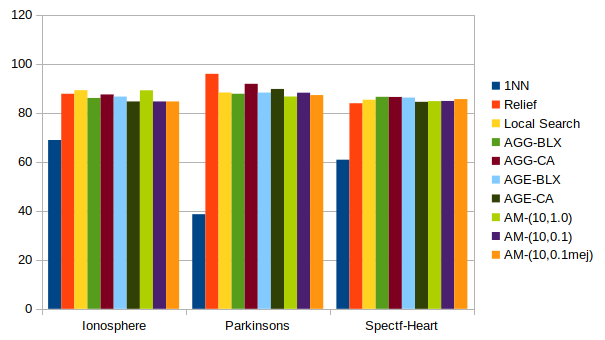
\includegraphics[width=0.65\textwidth]{images/tasa_clas.png}
		\caption{Tasa de clasificación.}
	\end{figure}

	Se observa que, a parte de 1NN, el resto de algoritmos proporcionan tasas de clasificación similares entre sí, dependiendo del dataset ganan unos u otros, no hay un patrón claro. Aunque Relief da buen resultado en un par de datasets tampoco es de mucho interés pues sabemos que no proporciona apenas tasa de reducción. Lo que sí podemos destacar es que tanto los algoritmos genéticos como meméticos han dado buenas tasas de clasificación, de hecho se han mejorado en Parkinsons y Spectf-Heart respecto a BL. En Ionosphere sigue ganando BL pero con una diferencia mínima a AM-(10,1.0). No se observa de forma consistente un mejor resultado de los algoritmos meméticos respecto a los genéticos, ni de los algoritmos generacionales respecto a los estacionarios, ni entre el cruce BLX y CA.~\\
	
	
	Vemos ahora las tasas de reducción:
	\begin{figure}[H]
		\centering
		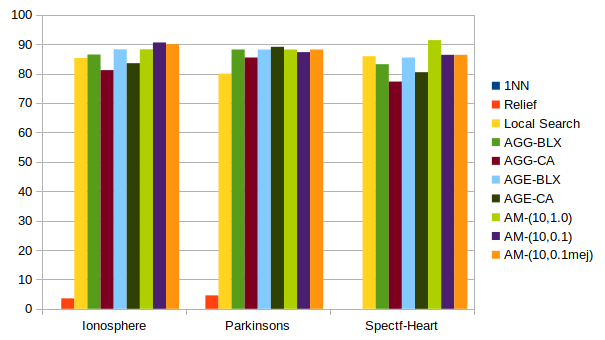
\includegraphics[width=0.65\textwidth]{images/tasa_red.png}
		\caption{Tasa de reducción.}
	\end{figure}
	
	Sabemos que BL era el que mejor resultado proporcionaba hasta el momento. Vemos que se han mejorado los resultados en los 3 datasets. A excepción de Parkinsons, que el mejor resultado lo proporciona AGE-CA, en el resto de datasets el mejor resultado viene dado por un algoritmo memético. Además vemos que se consigue mejor tasa de reducción con cruce BLX que con CA tanto en Ionosphere como Spect-Heart.~\\
	
	Por último el valor agregado:
	
	\begin{figure}[H]
		\centering
		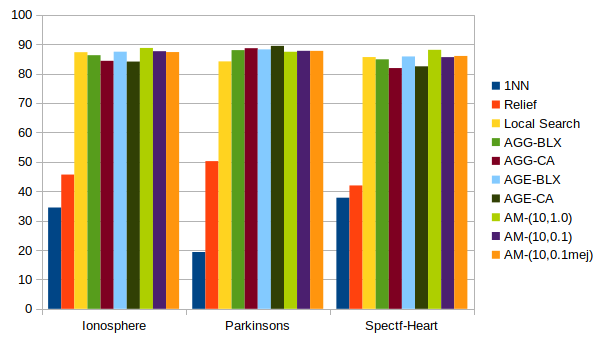
\includegraphics[width=0.65\textwidth]{images/agr.png}
		\caption{Valor de función objetivo o agregado.}
	\end{figure}
	
	De nuevo se han superado los resultados de BL en los 3 datasets. A excepción de Parkinsons, que es el datasets más pequeño, se observan ligeramente mejores resultados de los algoritmos meméticos respecto a los genéticos. Dedicar evaluaciones de la función objetivo a la búsqueda local tras cada generación ha resultado efectivo. Tanto en Ionosphere como Spect-Heart se tiene el mejor resultado con AM-(10,1.0), siendo mejor aplicar BL sobre toda la población; aumentando la exploración, y siendo todos los chromosomas mejores en cada generación de cara a la selección, cruce y mutación. Aún así cabe recalcar que no se observan de forma consistente ganadores y perdedores entre los meméticos, no hay mucha diferencia entre los valores de función objetivo obtenidos y las diferencias pueden deberse a la casuística del dataset o la propia aleatoriedad introducida. 
	
	Se observa en Ionosphere y Spectf-Heart mejor resultado de cruce BLX respecto CA, aunque esto se invierte en Parkinsons, no se observa una muy clara superioridad de BLX respecto CA. Realmente, tal y como se ha implementado CA, tanto BLX como CA son cruces con alta capacidad de exploración.
	
	Tanto los algoritmos genéticos generacionales como estacionarios proporcionan resultados similares. La alta presión selectiva del estacionario no ha supuesto una desventaja, de hecho AGE-BLX proporciona el mejor resultado de algoritmos generacionales tanto en Ionosphere como Spectf-Heart.~\\
	
	En cuanto a los tiempos de ejecución:
	
	
	\begin{figure}[H]
		\centering
		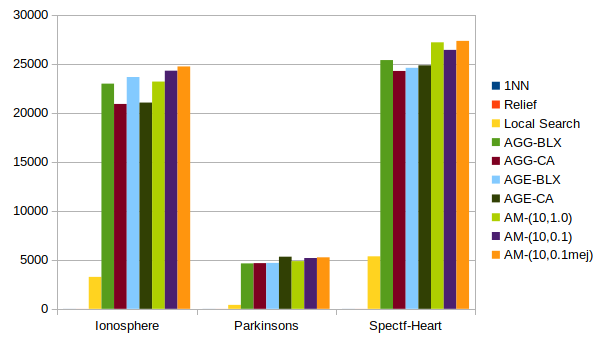
\includegraphics[width=0.65\textwidth]{images/time.png}
		\caption{Tiempos de ejecución.}
	\end{figure}
	
	Anteriormente BL era el algoritmo con mayor tiempo de ejecución. Ahora observamos una gran diferencia respecto BL: los algoritmos generacionales y meméticos suponen más de 4 veces el tiempo de BL, se ha requerido mucho tiempo para mejorar, y no por mucho, al resultado de BL. Los algoritmos genéticos tienen tiempos de ejecución similares entre sí. Sí se observa mayor tiempo de ejecución de los algoritmos meméticos respecto a genéticos ya que, aunque realizan las mismas evaluaciones de función objetivo, tienen como ``añadido'' las operaciones de la búsqueda local.~\\
		
	
	\subsection{Experimento extra:}
	
	Se ha decidido experimentar un nuevo operador de cruce, SBX (Simulated Binary Crossover), propuesto en 1995 por Deb y Agrawal. Este operador de cruce simula un cruce binario de un solo punto en variables reales. Para ello, dados dos padres $p_1(i)$ y $p_2(i)$, este cruce genera dos decendientes $d_1(i)$ y $d_2(i)$ dados por la siguiente expresión:
	
	$$c_1(i)=0.5[(1+\beta ) p_1(i) + (1-\beta)p_2(i)]$$
	$$c_2(i)=0.5[(1-\beta ) p_1(i) + (1+\beta)p_2(i)]$$

	donde $\beta$ es un factor de dispersión dado por
	
	$$\beta=\begin{cases}
		(2u)^{\frac{1}{\eta+1}} & u<0.5\\
		\left(\frac{1}{2(1-u)}\right)^{\frac{1}{\eta+1}} & u\geq 0.5
	\end{cases}$$
	donde $u\in \mathcal{U}(0,1)$, y $\eta \in \mathbb{R}^+$ es un parámetro dado.\\
	
	Para la implementación se ha decidido tomar $\eta=2$.
	
	Referencia: \url{https://content.wolfram.com/uploads/sites/13/2018/02/09-2-2.pdf}~\\
	
	Mostramos el pseudocódigo:
	\begin{algorithm}
	\caption{sbx2\_cross}
		\KwIn{Dos cromosomas $p1$ y $p2$}
		\KwOut{Los dos cromosomas descendientes $d1$ y $d2$}
		\Begin{
			$gen\_size \leftarrow p1.genes.size()$
			
			$\eta \leftarrow 2$
			
			$u\leftarrow random(0,1)$
			
			\If{$u < 0.5$}{
				$b\leftarrow 2u^{\frac{1}{\eta+1}}$
			}
			\Else{
				$b\leftarrow \frac{1}{2(1-u)}^{\frac{1}{\eta+1}}$
			}
			
			\For{$i=0$ \textbf{to} $gen\_size$}{
				
				$d1.genes[i] \leftarrow 0.5 * ( (1+b)*p1.genes[i] + (1-b)*p2.genes[i])$
				
				$d2.genes[i] \leftarrow 0.5 * ( (1-b)*p1.genes[i] + (1+b)*p2.genes[i])$
			
			}
			\tcp{para evitar evaluaciones de f.obj redundantes antes de la mutación}
			$d1.obj \leftarrow -1$
			
			$d2.obj \leftarrow -1$
			
			\Return{$d1$, $d2$}
		}
	\end{algorithm}
	
	Se muestran los resultados obtenidos para algoritmos genéticos y meméticos con cruce SBX2: ~\\
	
	\textbf{AGG-SBX2}
	
	\begin{tabbing}
	\resizebox{\textwidth}{!}{%
		\begin{tabular}{|c|}
			\hline \textbf{Nº}\\ \textbf{part.} 
			\\ \hline
			\textbf{P1} \\ \hline 
			\textbf{P2} \\ \hline
			\textbf{P3} \\ \hline 
			\textbf{P4} \\ \hline
			\textbf{P5} \\ \hline
			\textbf{Media} \\ \hline
		\end{tabular}
		\begin{tabular}{|c|c|c|c|}
			\hline
			\multicolumn{4}{|c|}{\textbf{Ionosphere}} \\ \hline
			\textbf{\%clas} & \textbf{\%red} & \textbf{Agr.} & \textbf{T} \\ \hline 
			83.0986 & 82.3529 & 82.7258 & 21359.2 \\ \hline
81.4286 & 85.2941 & 83.3613 & 19516.3 \\ \hline
92.8571 & 88.2353 & 90.5462 & 19828 \\ \hline
87.1429 & 82.3529 & 84.7479 & 20047.1 \\ \hline
91.4286 & 91.1765 & 91.3025 & 23429 \\ \hline
87.19116 & 85.88234 & 86.53674 & 20835.92 \\ \hline

		\end{tabular}
		
		\begin{tabular}{|c|c|c|c|}
			\hline
			\multicolumn{4}{|c|}{\textbf{Parkinsons}} \\ \hline
			\textbf{\%clas} & \textbf{\%red} & \textbf{Agr.} & \textbf{T} \\ \hline 
			95 & 77.2727 & 86.1364 & 4173.41 \\ \hline
100 & 72.7273 & 86.3636 & 5158.73 \\ \hline
82.0513 & 81.8182 & 81.9347 & 4301.68 \\ \hline
94.7368 & 81.8182 & 88.2775 & 5413.85 \\ \hline
86.8421 & 90.9091 & 88.8756 & 5938.4 \\ \hline
91.72604 & 80.9091 & 86.31756 & 4997.214 \\ \hline

		\end{tabular}
		
		\begin{tabular}{|c|c|c|c|}
			\hline
			\multicolumn{4}{|c|}{\textbf{Spectf-Heart}} \\ \hline
			\textbf{\%clas} & \textbf{\%red} & \textbf{Agr.} & \textbf{T} \\ \hline 
			90 & 86.3636 & 88.1818 & 24516.1 \\ \hline
87.1429 & 77.2727 & 82.2078 & 23955.1 \\ \hline
85.7143 & 81.8182 & 83.7662 & 24019.5 \\ \hline
88.5714 & 77.2727 & 82.9221 & 24072.4 \\ \hline
89.7059 & 75 & 82.3529 & 25851.1 \\ \hline
88.2269 & 79.54544 & 83.88616 & 24482.84 \\ \hline
		\end{tabular}
		}
	\end{tabbing}
	

	
	\textbf{AGE-SBX2}	
	
	\begin{tabbing}
	\resizebox{\textwidth}{!}{%
		\begin{tabular}{|c|}
			\hline \textbf{Nº}\\ \textbf{part.} 
			\\ \hline
			\textbf{P1} \\ \hline 
			\textbf{P2} \\ \hline
			\textbf{P3} \\ \hline 
			\textbf{P4} \\ \hline
			\textbf{P5} \\ \hline
			\textbf{Media} \\ \hline
		\end{tabular}
		\begin{tabular}{|c|c|c|c|}
			\hline
			\multicolumn{4}{|c|}{\textbf{Ionosphere}} \\ \hline
			\textbf{\%clas} & \textbf{\%red} & \textbf{Agr.} & \textbf{T} \\ \hline 
			90.1408 & 85.2941 & 87.7175 & 19900.6 \\ \hline
85.7143 & 79.4118 & 82.563 & 21885 \\ \hline
92.8571 & 79.4118 & 86.1345 & 19431.4 \\ \hline
87.1429 & 85.2941 & 86.2185 & 19550.2 \\ \hline
88.5714 & 82.3529 & 85.4622 & 19500.6 \\ \hline
88.8853 & 82.35294 & 85.61914 & 20053.56 \\ \hline

		\end{tabular}
		
		\begin{tabular}{|c|c|c|c|}
			\hline
			\multicolumn{4}{|c|}{\textbf{Parkinsons}} \\ \hline
			\textbf{\%clas} & \textbf{\%red} & \textbf{Agr.} & \textbf{T} \\ \hline 
			92.5 & 72.7273 & 82.6136 & 5232.04 \\ \hline
70 & 86.3636 & 78.1818 & 5331.24 \\ \hline
89.7436 & 72.7273 & 81.2354 & 5167.61 \\ \hline
92.1053 & 77.2727 & 84.689 & 4325.87 \\ \hline
89.4737 & 81.8182 & 85.6459 & 5314.16 \\ \hline
86.76452 & 78.18182 & 82.47314 & 5074.184 \\ \hline

		\end{tabular}
		
		\begin{tabular}{|c|c|c|c|}
			\hline
			\multicolumn{4}{|c|}{\textbf{Spectf-Heart}} \\ \hline
			\textbf{\%clas} & \textbf{\%red} & \textbf{Agr.} & \textbf{T} \\ \hline 
			84.2857 & 70.4545 & 77.3701 & 24378 \\ \hline
90 & 70.4545 & 80.2273 & 25355.3 \\ \hline
87.1429 & 70.4545 & 78.7987 & 24750.8 \\ \hline
92.8571 & 68.1818 & 80.5195 & 23929.5 \\ \hline
79.4118 & 75 & 77.2059 & 24308.7 \\ \hline
86.7395 & 70.90906 & 78.8243 & 24544.46 \\ \hline
		\end{tabular}
		}
	\end{tabbing}
	
	\textbf{AM-(10,1.0)-SBX2}	
	
	\begin{tabbing}
	\resizebox{\textwidth}{!}{%
		\begin{tabular}{|c|}
			\hline \textbf{Nº}\\ \textbf{part.} 
			\\ \hline
			\textbf{P1} \\ \hline 
			\textbf{P2} \\ \hline
			\textbf{P3} \\ \hline 
			\textbf{P4} \\ \hline
			\textbf{P5} \\ \hline
			\textbf{Media} \\ \hline
		\end{tabular}
		\begin{tabular}{|c|c|c|c|}
			\hline
			\multicolumn{4}{|c|}{\textbf{Ionosphere}} \\ \hline
			\textbf{\%clas} & \textbf{\%red} & \textbf{Agr.} & \textbf{T} \\ \hline 
			92.9577 & 91.1765 & 92.0671 & 22639.4 \\ \hline
84.2857 & 91.1765 & 87.7311 & 20164.6 \\ \hline
88.5714 & 91.1765 & 89.8739 & 23002.2 \\ \hline
94.2857 & 88.2353 & 91.2605 & 19438.2 \\ \hline
85.7143 & 88.2353 & 86.9748 & 21609 \\ \hline
89.16296 & 90.00002 & 89.58148 & 21370.68 \\ \hline

		\end{tabular}
		
		\begin{tabular}{|c|c|c|c|}
			\hline
			\multicolumn{4}{|c|}{\textbf{Parkinsons}} \\ \hline
			\textbf{\%clas} & \textbf{\%red} & \textbf{Agr.} & \textbf{T} \\ \hline 
			82.5 & 86.3636 & 84.4318 & 4229.03 \\ \hline
95 & 86.3636 & 90.6818 & 4280.44 \\ \hline
94.8718 & 90.9091 & 92.8904 & 5098 \\ \hline
81.5789 & 90.9091 & 86.244 & 4389.35 \\ \hline
94.7368 & 90.9091 & 92.823 & 5108.6 \\ \hline
89.7375 & 89.0909 & 89.4142 & 4621.084 \\ \hline

		\end{tabular}
		
		\begin{tabular}{|c|c|c|c|}
			\hline
			\multicolumn{4}{|c|}{\textbf{Spectf-Heart}} \\ \hline
			\textbf{\%clas} & \textbf{\%red} & \textbf{Agr.} & \textbf{T} \\ \hline 
			88.5714 & 88.6364 & 88.6039 & 26515.3 \\ \hline
81.4286 & 88.6364 & 85.0325 & 26422.7 \\ \hline
82.8571 & 88.6364 & 85.7468 & 28527.5 \\ \hline
88.5714 & 86.3636 & 87.4675 & 24712.1 \\ \hline
80.8824 & 79.5455 & 80.2139 & 24506.5 \\ \hline
84.46218 & 86.36366 & 85.41292 & 26136.82 \\ \hline
		\end{tabular}
		}
	\end{tabbing}
	
	\textbf{AM-(10,0.1)-SBX2}	
	
	\begin{tabbing}
	\resizebox{\textwidth}{!}{%
		\begin{tabular}{|c|}
			\hline \textbf{Nº}\\ \textbf{part.} 
			\\ \hline
			\textbf{P1} \\ \hline 
			\textbf{P2} \\ \hline
			\textbf{P3} \\ \hline 
			\textbf{P4} \\ \hline
			\textbf{P5} \\ \hline
			\textbf{Media} \\ \hline
		\end{tabular}
		\begin{tabular}{|c|c|c|c|}
			\hline
			\multicolumn{4}{|c|}{\textbf{Ionosphere}} \\ \hline
			\textbf{\%clas} & \textbf{\%red} & \textbf{Agr.} & \textbf{T} \\ \hline 
			90.1408 & 91.1765 & 90.6587 & 19940 \\ \hline
87.1429 & 91.1765 & 89.1597 & 21074.3 \\ \hline
87.1429 & 91.1765 & 89.1597 & 21811.7 \\ \hline
87.1429 & 91.1765 & 89.1597 & 21474.9 \\ \hline
82.8571 & 91.1765 & 87.0168 & 23074 \\ \hline
86.88532 & 91.1765 & 89.03092 & 21474.98 \\ \hline

		\end{tabular}
		
		\begin{tabular}{|c|c|c|c|}
			\hline
			\multicolumn{4}{|c|}{\textbf{Parkinsons}} \\ \hline
			\textbf{\%clas} & \textbf{\%red} & \textbf{Agr.} & \textbf{T} \\ \hline 
			72.5 & 90.9091 & 81.7045 & 4274.03 \\ \hline
95 & 90.9091 & 92.9545 & 5859.17 \\ \hline
94.8718 & 90.9091 & 92.8904 & 5487.99 \\ \hline
92.1053 & 90.9091 & 91.5072 & 5938.07 \\ \hline
92.1053 & 90.9091 & 91.5072 & 5880.71 \\ \hline
89.31648 & 90.9091 & 90.11276 & 5487.994 \\ \hline

		\end{tabular}
		
		\begin{tabular}{|c|c|c|c|}
			\hline
			\multicolumn{4}{|c|}{\textbf{Spectf-Heart}} \\ \hline
			\textbf{\%clas} & \textbf{\%red} & \textbf{Agr.} & \textbf{T} \\ \hline 
			81.4286 & 86.3636 & 83.8961 & 24603.2 \\ \hline
80 & 93.1818 & 86.5909 & 25159.7 \\ \hline
88.5714 & 88.6364 & 88.6039 & 24903.2 \\ \hline
81.4286 & 86.3636 & 83.8961 & 24152.5 \\ \hline
77.9412 & 81.8182 & 79.8797 & 24326.7 \\ \hline
81.87396 & 87.27272 & 84.57334 & 24629.06 \\ \hline
		\end{tabular}
		}
	\end{tabbing}
	
	\textbf{AM-(10,0.1mej)-SBX2}	
	
	\begin{tabbing}
	\resizebox{\textwidth}{!}{%
		\begin{tabular}{|c|}
			\hline \textbf{Nº}\\ \textbf{part.} 
			\\ \hline
			\textbf{P1} \\ \hline 
			\textbf{P2} \\ \hline
			\textbf{P3} \\ \hline 
			\textbf{P4} \\ \hline
			\textbf{P5} \\ \hline
			\textbf{Media} \\ \hline
		\end{tabular}
		\begin{tabular}{|c|c|c|c|}
			\hline
			\multicolumn{4}{|c|}{\textbf{Ionosphere}} \\ \hline
			\textbf{\%clas} & \textbf{\%red} & \textbf{Agr.} & \textbf{T} \\ \hline 
			87.3239 & 88.2353 & 87.7796 & 19999.1 \\ \hline
82.8571 & 91.1765 & 87.0168 & 20578.1 \\ \hline
82.8571 & 88.2353 & 85.5462 & 22925.2 \\ \hline
92.8571 & 91.1765 & 92.0168 & 22993.9 \\ \hline
81.4286 & 88.2353 & 84.8319 & 19575.8 \\ \hline
85.46476 & 89.41178 & 87.43826 & 21214.42 \\ \hline

		\end{tabular}
		
		\begin{tabular}{|c|c|c|c|}
			\hline
			\multicolumn{4}{|c|}{\textbf{Parkinsons}} \\ \hline
			\textbf{\%clas} & \textbf{\%red} & \textbf{Agr.} & \textbf{T} \\ \hline 
			87.5 & 81.8182 & 84.6591 & 4282 \\ \hline
87.5 & 86.3636 & 86.9318 & 4264.69 \\ \hline
84.6154 & 86.3636 & 85.4895 & 4343.89 \\ \hline
92.1053 & 90.9091 & 91.5072 & 5917.92 \\ \hline
78.9474 & 86.3636 & 82.6555 & 4868.58 \\ \hline
86.13362 & 86.36362 & 86.24862 & 4735.416 \\ \hline

		\end{tabular}
		
		\begin{tabular}{|c|c|c|c|}
			\hline
			\multicolumn{4}{|c|}{\textbf{Spectf-Heart}} \\ \hline
			\textbf{\%clas} & \textbf{\%red} & \textbf{Agr.} & \textbf{T} \\ \hline 
			80 & 93.1818 & 86.5909 & 27844 \\ \hline
78.5714 & 84.0909 & 81.3312 & 27425.5 \\ \hline
78.5714 & 79.5455 & 79.0584 & 27507.6 \\ \hline
87.1429 & 90.9091 & 89.026 & 27381.2 \\ \hline
86.7647 & 86.3636 & 86.5642 & 26928 \\ \hline
82.21008 & 86.81818 & 84.51414 & 27417.26 \\ \hline
		\end{tabular}
		}
	\end{tabbing}
	
	
	Se muestra la tabla resumen:
	
	\begin{tabbing}
	\resizebox{\textwidth}{!}{%
		\begin{tabular}{|c|}
			\hline \textbf{Nº}\\ \textbf{part.} 
			\\ \hline
			\textbf{1-NN} \\ \hline 
			\textbf{Relief} \\ \hline
			\textbf{BL} \\ \hline 
			\textbf{AGG-BLX} \\ \hline
			\textbf{AGG-CA} \\ \hline
			\textbf{AGE-BLX} \\ \hline
			\textbf{AGE-CA} \\ \hline
			\textbf{AM-(10,1.0)} \\ \hline
			\textbf{AM-(10,0.1)} \\ \hline
			\textbf{AM-(10,0.1mej)} \\ \hline
			\textbf{AGG-SBX2} \\ \hline
			\textbf{AGE-SBX2} \\ \hline
			\textbf{AM-(10,1.0)-SBX2} \\ \hline
			\textbf{AM-(10,0.1)-SBX2} \\ \hline
			\textbf{AM-(10,0.1mej)-SBX2} \\ \hline
		\end{tabular}
		\begin{tabular}{|c|c|c|c|}
			\hline
			\multicolumn{4}{|c|}{\textbf{Ionosphere}} \\ \hline
			\textbf{\%clas} & \textbf{\%red} & \textbf{Agr.} & \textbf{T} \\ \hline 
			68.89334	&0	          &34.44672	&0.3458\\ \hline
87.74648&	3.529414	  &45.63794	&1.7594\\ \hline
89.2032	  &85.2941	    &87.24868	&3255.044\\ \hline
86.04024 & 86.47058 & 86.25542 & 22970.16\\ \hline
87.46882 & 81.17646 & 84.32264 & 20903.28\\ \hline
86.61974 & 88.2353 & 87.4275 & 23650.94\\ \hline
84.6197 & 83.5294 & 84.07456 & 21042.54\\ \hline
89.17104 & 88.2353 & \textbf{88.70318} & 23181.3\\ \hline
84.61168 & 90.58826 & 87.59996 & 24288.08\\ \hline
84.6197 & 90.00002 & 87.30984 & 24726.3\\ \hline
87.19116 & 85.88234 & 86.53674 & 20835.92 \\ \hline
88.8853 & 82.35294 & 85.61914 & 20053.56 \\ \hline
89.16296 & 90.00002 & \textcolor{blue}{89.58148} & 21370.68 \\ \hline
86.88532 & 91.1765 & 89.03092 & 21474.98 \\ \hline
85.46476 & 89.41178 & 87.43826 & 21214.42 \\ \hline
		\end{tabular}
		
		\begin{tabular}{|c|c|c|c|}
			\hline
			\multicolumn{4}{|c|}{\textbf{Parkinsons}} \\ \hline
			\textbf{\%clas} & \textbf{\%red} & \textbf{Agr.} & \textbf{T} \\ \hline 
			38.60188	&0	        &19.30094	&0.0934\\ \hline
95.89542&	4.545452	&50.22044	&0.3688\\ \hline
88.278	 & 79.99998	&84.139	  &396.8584\\ \hline
87.76384 & 88.1818 & 87.97282 & 4628.332\\ \hline
91.80432 & 85.45454 & 88.62944 & 4654.054\\ \hline
88.2517 & 88.18182 & 88.21672 & 4683.564\\ \hline
89.72538 & 89.0909 & \textbf{89.40814} & 5315.516\\ \hline
86.63292 & 88.18182 & 87.40736 & 4859.698\\ \hline
88.18556 & 87.27272 & 87.72914 & 5184.384\\ \hline
87.21256 & 88.1818 & 87.69718 & 5253.436\\ \hline
91.72604 & 80.9091 & 86.31756 & 4997.214 \\ \hline
86.76452 & 78.18182 & 82.47314 & 5074.184 \\ \hline
89.7375 & 89.0909 & 89.4142 & 4621.084 \\ \hline
89.31648 & 90.9091 & \textcolor{blue}{90.11276} & 5487.994 \\ \hline
86.13362 & 86.36362 & 86.24862 & 4735.416 \\ \hline

		\end{tabular}
		
		\begin{tabular}{|c|c|c|c|}
			\hline
			\multicolumn{4}{|c|}{\textbf{Spectf-Heart}} \\ \hline
			\textbf{\%clas} & \textbf{\%red} & \textbf{Agr.} & \textbf{T} \\ \hline 
			75.563	  &0	      &37.78152	&0.4114\\ \hline
83.87396	&0	      &41.93698	&2.2224\\ \hline
85.31934	&85.9091	&85.61422	&5350.368\\ \hline
86.5126 & 83.18182 & 84.84722 & 25376.7\\ \hline
86.4622 & 77.27276 & 81.86746 & 24268.34\\ \hline
86.2101 & 85.45456 & 85.8323 & 24587.5\\ \hline
84.47058 & 80.45454 & 82.46258 & 24840.7\\ \hline
84.75628 & 91.36364 & \textbf{88.05998} & 27185.14\\ \hline
84.8067 & 86.36364 & 85.5852 & 26415.84\\ \hline
85.59666 & 86.36362 & 85.98012 & 27331\\ \hline
88.2269 & 79.54544 & 83.88616 & 24482.84 \\ \hline
86.7395 & 70.90906 & 78.8243 & 24544.46 \\ \hline
84.46218 & 86.36366 & \textcolor{blue}{85.41292} & 26136.82 \\ \hline
81.87396 & 87.27272 & 84.57334 & 24629.06 \\ \hline
82.21008 & 86.81818 & 84.51414 & 27417.26 \\ \hline
		\end{tabular}
		}
	\end{tabbing}~\\
	
	Se ha marcado en azul el mejor resultado con cruce SBX2.\\
	
	 Los resultados han sido buenos, aunque hay cierta influencia por el dataset; en Ionosphere y Parkinsons se ha obtenido nuevo máximo en función objetivo, en Spectf-Heart sin embargo no consigue mejorar los resultados.
	
	Aunque haya marcado máximos no parece claro que sea mejor que el cruce BLX o AC, en los algoritmos genéticos no muestra ser superior a BLX o AC.
	
	Desde luego sí que funciona y parece otro tipo de cruce que podría considerarse.

\end{document}
	

